%-------------------------------------------------------------------------------------------------------
%
%
%
%-------------------------------------------------------------------------------------------------------
\documentclass[a4paper, 12pt]{book}  

%-------------------------------------------------------------------------------------------------------
% Packages
%
%-------------------------------------------------------------------------------------------------------
\usepackage{amsmath}           
\usepackage{hyperref}           
\usepackage{geometry}           
\usepackage{fancyhdr}           
\usepackage{titlesec}
\usepackage{titlepic}
\usepackage{booktabs}
\usepackage[all]{nowidow}      
\usepackage{listings}
\usepackage{xcolor}
\usepackage{tcolorbox}
\usepackage{graphicx}           
\usepackage{pdfpages}
\usepackage{float}
\usepackage{placeins}
\usepackage{tikz}

%-------------------------------------------------------------------------------------------------------
% Directory paths used for included files
%
%-------------------------------------------------------------------------------------------------------
% file dir path
%
\newcommand{\srcinputpath}{../../LcsNodes-Pico/}
%
% Usage:
%
%\includegraphics{\inputpath imagefile.pdf}


%-------------------------------------------------------------------------------------------------------
% Chapter title settings 
%
%-------------------------------------------------------------------------------------------------------
\titleformat{\chapter}[hang]{\normalfont\huge\bfseries}{\thechapter}{2pc}{}
\titlespacing*{\chapter}{0pt}{0.1in}{0.2in}

%-------------------------------------------------------------------------------------------------------
% Page layout settings
%
%-------------------------------------------------------------------------------------------------------
\geometry{a4paper, margin=1in, top=1in, bottom=1in, left=1in, right=1in, headheight=0.5in}
\addtolength{\parskip}{1.0ex}

%-------------------------------------------------------------------------------------------------------
% Page numbering settings
%
%-------------------------------------------------------------------------------------------------------
\pagestyle{fancy}               
\fancyhf{}                     
\fancyhead[L]{\leftmark}       
\fancyfoot[R]{\thepage}         
\renewcommand{\headrulewidth}{0pt}
\renewcommand{\footrulewidth}{0pt}

%-------------------------------------------------------------------------------------------------------
% Listing style for showing source code files
%
%-------------------------------------------------------------------------------------------------------
\lstdefinestyle{listingstyle}{ 
    backgroundcolor=\color{gray!10}, 
    basicstyle=\ttfamily\tiny,
    keywordstyle=\color{magenta},
    identifierstyle=\ttfamily\color{blue},
    numberstyle=\tiny\color{gray},
    commentstyle=\ttfamily\color{teal},
    showstringspaces=false,
    numbers=left,
    frame=sigle
} 

%-------------------------------------------------------------------------------------------------------
% Document start
%
%-------------------------------------------------------------------------------------------------------
\begin{document}

    \begin{center}
        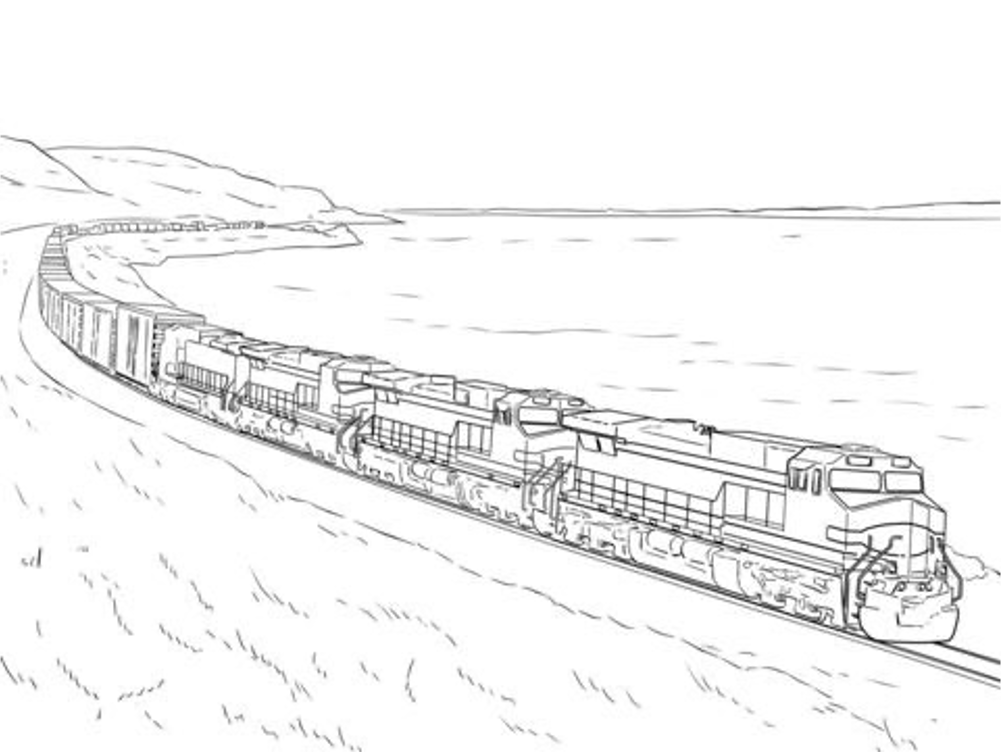
\includegraphics[width=0.7\textwidth]{./figures/Frontpage-Picture.png}

        \vspace{ 2cm }
        {\Huge \textbf{A Layout Control System for \\ Model Railroads}} 

        \vspace{ 2cm }
        {\Large Helmut Fieres}

        {\large \today}
    \end{center}

    \frontmatter            
    \tableofcontents         

    \mainmatter             
    \chapter{Introduction}

Model railroading. A fascinating hobby with many different facets. While some hobbyist would just like to watch trains running, others dive deeper into parts of their hobby. Some build a realistic scenery and model a certain time era with realistic operations. Others build locos and rolling equipment from scratch. Yet others enjoy the basic benchwork building, electrical aspects of wiring and control. They all have in common that they truly enjoy their hobby.

This little book is about the hardware and software of a layout control system for managing a model railroad layout. Controlling a layout is as old as the hobby itself. I remember my first model railroad. A small circle with one turnout, a little steam engine and three cars. Everything was reachable by hand, a single transformer supplied the current to the locomotive. As more turnouts were added, the arm was not long enough any more, simple switches, electrical turnouts and some control wires came to the rescue. Over time one locomotive did not stay alone, others joined. Unfortunately, being analog engines, they could only be controlled by electric current to the track. The layout was thus divided into electrical sections. And so on and so on. Before you know it, quite some cabling and simple electrical gear was necessary.

Nearly four decades ago, locomotives, turnouts, signals and other devices on the layout became digital. With growing sophistication, miniaturization and the requirement to model operations closer and closer to the real railroad, layout control became a hobby in itself. Today, locomotives are running computers on wheels far more capable than computers that used to fill entire rooms. Not to mention the pricing. Turnout control and track occupancy detection all fed into a digital control system, allowing for very realistic operations.

The demands for a layout control system can be divided into three areas. The first area is of course {\bf running} locomotives. This is what it should be all about, right? Many locomotives need to be controlled simultaneously. Also, locomotives need to be grouped into consists for large trains, such as for example a long freight train with four diesel engines and fifty boxcars. Next are the two areas {\bf observe} and {\bf act}. Track occupancy detection is a key requirement for running multiple locomotives and knowing where they are. But also, knowing which way a turnout is set, the current consumption of a track section are good examples for layout observation. Following observation is to act on the information gathered. Setting turnouts and signals or enabling a track section are good examples for acting on an observation.

Running, observing an acting requires some form of {\bf configurations} and {\bf operations} What used to be a single transformer, some cabling and switches has turned into computer controlled layout with many devices and one or more bus systems. Sophisticated layouts need a way to configure the locomotives, devices and manage operations of layouts. Enter the world of digital control and computers.

After several decades, there is today a rich set of product offerings and standards available. There are many vendors offering hardware and software components as well as entire systems. Unfortunately they are often not compatible with each other. Furthermore, engaged open software communities took on to build do it yourself systems more or less compatible with vendors in one or the other way. There is a lively community of hardware and software designers building hardware and software layout control systems more or less from scratch or combined using existing industry products.

\section{Elements of a Layout Control System}

Before diving into concept and implementation details, let's first outline what is needed and what the resulting key requirements are. Above all, our layout control system should be capable to simultaneously run locomotives and manage all devices, such as turnouts and signals, on the layout. The system should be easy to expand as new ideas and requirements surface that need to be integrated without major incompatibilities to what was already built.

Having said that, we would need at least a {\bf base station}. This central component is the heart of most systems. A base station needs to be able to manage the running locomotives and to produce the DCC signals for the track where the running locomotive is. There are two main DCC signals to generate. One for the main track or track sections and one for the programming track. This is the track where a locomotive decoder can be configured. A base station could also be the place to keep a dictionary of all known locomotives and their characteristics. In addition to interfaces to issues commands for the running locomotives, there also need to be a way to configure the rolling stock.

Complementing the base station is the {\bf booster} or {\bf block controller} component that produce the electrical current for a track section. The booster should also monitor the current consumption to detect electrical shortages. Boosters comes in several ranges from providing the current for the smaller model scales as well as the larger model scales which can draw quite a few amps. There could be many boosters, one for each track section. The base station provides the signals for all of them.

The {\bf cab handheld} is the controlling device for a locomotive. Once a session is established, the control knobs and buttons are used to run the locomotive. Depending on the engine model, one could imagine a range of handhelds from rather simple handhelds just offering a speed dial and a few buttons up to a sophisticated handheld that mimics for example a diesel engine cab throttle stand.

With these three elements in place and a communication method between them, we are in business to run engines. Let's look at the communication method. Between the components, called nodes, there needs to be a {\bf communication bus} that transmits the commands between them. While the bus technology itself is not necessarily fixed, the messaging model implemented on top is. The bus itself has no master, any node can communicate with any other node by broadcasting a message, observed by all other nodes. Events that are broadcasted between the nodes play a central role. Any node can produce events, any node can consume events. Base station, boosters and handhelds are just nodes on this bus.

But layouts still need more. There are {\bf signals}, {\bf turnouts} and {\bf track detectors} as well as {\bf LEDs}, {\bf switches}, {\bf buttons} and a whole lot more things to imagine. They all need to be connected to the common messaging bus. The layout control system needs to provide not only the hardware interfaces and core firmware for the various device types to connect, it needs to also provide a great flexibility to configure the interaction between them. Pushing for example a button on a control field should result in a turnout being set, or even a set of turnouts to guide a train through a freight-yard and so on.

Especially on larger layouts, {\bf configuration} becomes quite an undertaking. The {\bf configuration model} should therefore be easy and intuitive to understand. The elements to configure should all follow the same operation principles and be extensible for specific functions. A computer is required for configuration. Once configured however, the computer is not required for operations. The capacity, i.e. the number of locomotives, signals, turnouts and other devices managed should be in the thousands.

Configuration as well as operations should be possible through sending the defined messages as well as a simple ASCII commands send to the base station which in turn generates the messages to broadcast via the common bus. A computer with a graphical UI would connect via the USB serial interface using the text commands.

\section{Standards, Components and Compatibility}

The DCC family of standards is the overall guiding standard. The layout system assumes the usage of DCC locomotive decoder equipped running gear and DCC stationary decoder accessories. Beyond this set of standards, it is not a requirement to be compatible with other model railroad electronic products and communication protocols. This does however not preclude gateways to interact in one form or another with such systems. Am example is to connect to a LocoNet system via a gateway node. Right now, this is not in scope for our first layout system.

All of the project should be well documented. One part of documentation is this book, the other part is the thoroughly commented LCS core library and all software components built on top. Each lesson learned, each decision taken, each tradeoff made is noted, and should help to understand the design approach taken. Imagine a fast forward of a couple of years. Without proper documentation it will be hard to remember how the whole system works and how it can be maintained and enhanced.

With respect to the components used, it uses as much as possible off the shelf electronic parts, such as readily available microcontrollers and their software stack as well as electronic parts in SMD and non-SMD form, for building parts of the system. The concepts should not restrict the development to build it all from scratch. It should however also be possible to use more integrated elements, such as a controller board and perhaps some matching shields, to also build a hardware module.

\section{This Book}

This book will describe my version of a layout control system with hardware and software designed from the ground up. The big question is why build one yourself. Why yet another one? There is after all no shortage on such systems readily available. And there are great communities out there already underway. The key reason for doing it yourself is that it is simply fun and you learn a lot about standards, electronics and programming by building a system that you truly understanding from the ground up. To say it with the words of Richard Feynman

\begin{quotation}
    \textit{ "What I cannot create, I do not understand. -- Richard Feynman"}
\end{quotation}

Although it takes certainly longer to build such a system from the ground up, you still get to play with the railroad eventually. And even after years, you will have a lay  out control system properly documented and easy to support and enhance further. Not convinced? Well, at least this book should be interesting and give some ideas and references how to go after building such a system.

\section{Parts and Chapters}

The book is organized into several parts and chapters. The first chapters describe the underlying concepts of the layout control system. Hardware modules, nodes, ports and events and their interaction are outlined. Next, the set of message that are transmitted between the components and the message protocol flow illustrate how the whole system interacts. With the concepts in place, the software library available to the node firmware programmer is explained along with example code snippets. After this section, we all have a good idea how the system configuration and operation works. The section is rounded up with a set of concrete programming examples.

Perhaps the most important part of a layout control system is the management of locomotives and track power. After all, we want to run engines and play. Our system is using the DCC standard for running locomotives and consequently DCC signals need to be generated for configuring and operating an engine. A base station module will manage the locomotive sessions, generating the respective DCC packets to transmit to the track. Layouts may consist of a number of track sections for which a hardware module is needed to manage the track power and monitor the power consumption. Finally, decoders can communicate back and track power modules need to be able to detect this communication. Two chapters will describe these two parts in great detail.

The next big part of the book starts with the hardware design of modules. First the overall outline of a hardware module and our approach to module design is discussed. Building a hardware module will rest on common building blocks such as a CAN bus interface, a microcontroller core, H-Bridges for DCC track signal generation and so on. Using a modular approach the section will describe the building blocks developed so far. It is the idea to combine them for the purpose of the hardware module.

With the concepts, the messages and protocol, the software library and the hardware building blocks in place, we are ready to actually build the necessary hardware modules. The most important module is the base station. Next are boosters, block controllers, handhelds, sensor and actor modules, and so on. Finally, there are also utility components such as monitoring the DCC packets on the track, that are described in the later chapters. Each major module is devoted a chapter that describes the hardware building blocks used, additional hardware perhaps needed, and the firmware developed on top of the core library specifically for the module. Finally, there are several appendices with reference information and further links and other information.

\section{A final note}

A final note. "Truly from the ground up" does not mean to really build it all yourself. As said, there are standards to follow and not every piece of hardware needs to be built from individual parts. There are many DCC decoders available for locomotives, let's not overdo it and just use them. There are also quite powerful controller boards along with great software libraries for the micro controllers, such as the CAN bus library for the AtMega Controller family, already available. There is no need to dive into all these details.

The design allows for building your own hardware just using of the shelf electronic components or start a little more integrated by using a controller board and other breakout boards. The book will however describe modules from the ground up and not use controller boards or shields. This way the principles are easier to see. The appendix section provides further information and links on how to build a system with some of the shelf parts instead of building it all yourself. With the concepts and software explained, it should not be a big issue to build your own mix of hardware and software.

I have added most of the source files in the appendix for direct reference. They can also be found also on GitHub. ( Note: still to do... ) Every building block schematic shown was used and tested in one component or another. However, sometimes the book may not exactly match the material found on the web or be slightly different until the next revision is completed. Still, looking at portions of the source in the text explain quite well what it will do. As said, it is the documentation that hopefully in a couple of years from now still tells you what was done so you can adapt and build upon it. And troubleshoot.

The book hopefully also helps anybody new to the whole subject with good background and starting pointers to build such a system. I also have looked at other peoples great work, which helped a lot. What I however also found is that often there are rather few comments or explanations in the source and you have to partially reverse engineer what was actually build for understanding how things work. For those who simply want to use an end product, just fine. There is nothing wrong with this approach. For those who want to truly understand, it offers nevertheless little help. I hope to close some of these gaps with a well documented layout system and its inner workings.

In the end, as with any hobby, the journey is the goal. The reward in this undertaking is to learn about the digital control of model railroads from running a simple engine to a highly automated layout with one set of software and easy to build and use hardware components. Furthermore, it is to learn about how to build a track signaling system that manages analog and digital engines at the same time. So, enjoy.




    %-------------------------------------------------------------------------------------------------------
%
%
%
%-------------------------------------------------------------------------------------------------------    
\chapter{General Concepts}

At a higher level, the layout control system consists of components and a communication scheme. This chapter will define the key concepts of a layout system. At the heart of the layout control system is a common communication bus to which all modules connect. The others key elements are node, events, ports and attributes. Let's define these items first and then talk about how they interact. The following figure depicts the high level view of a layout control system.

\begin{figure}[h]
    \centering
    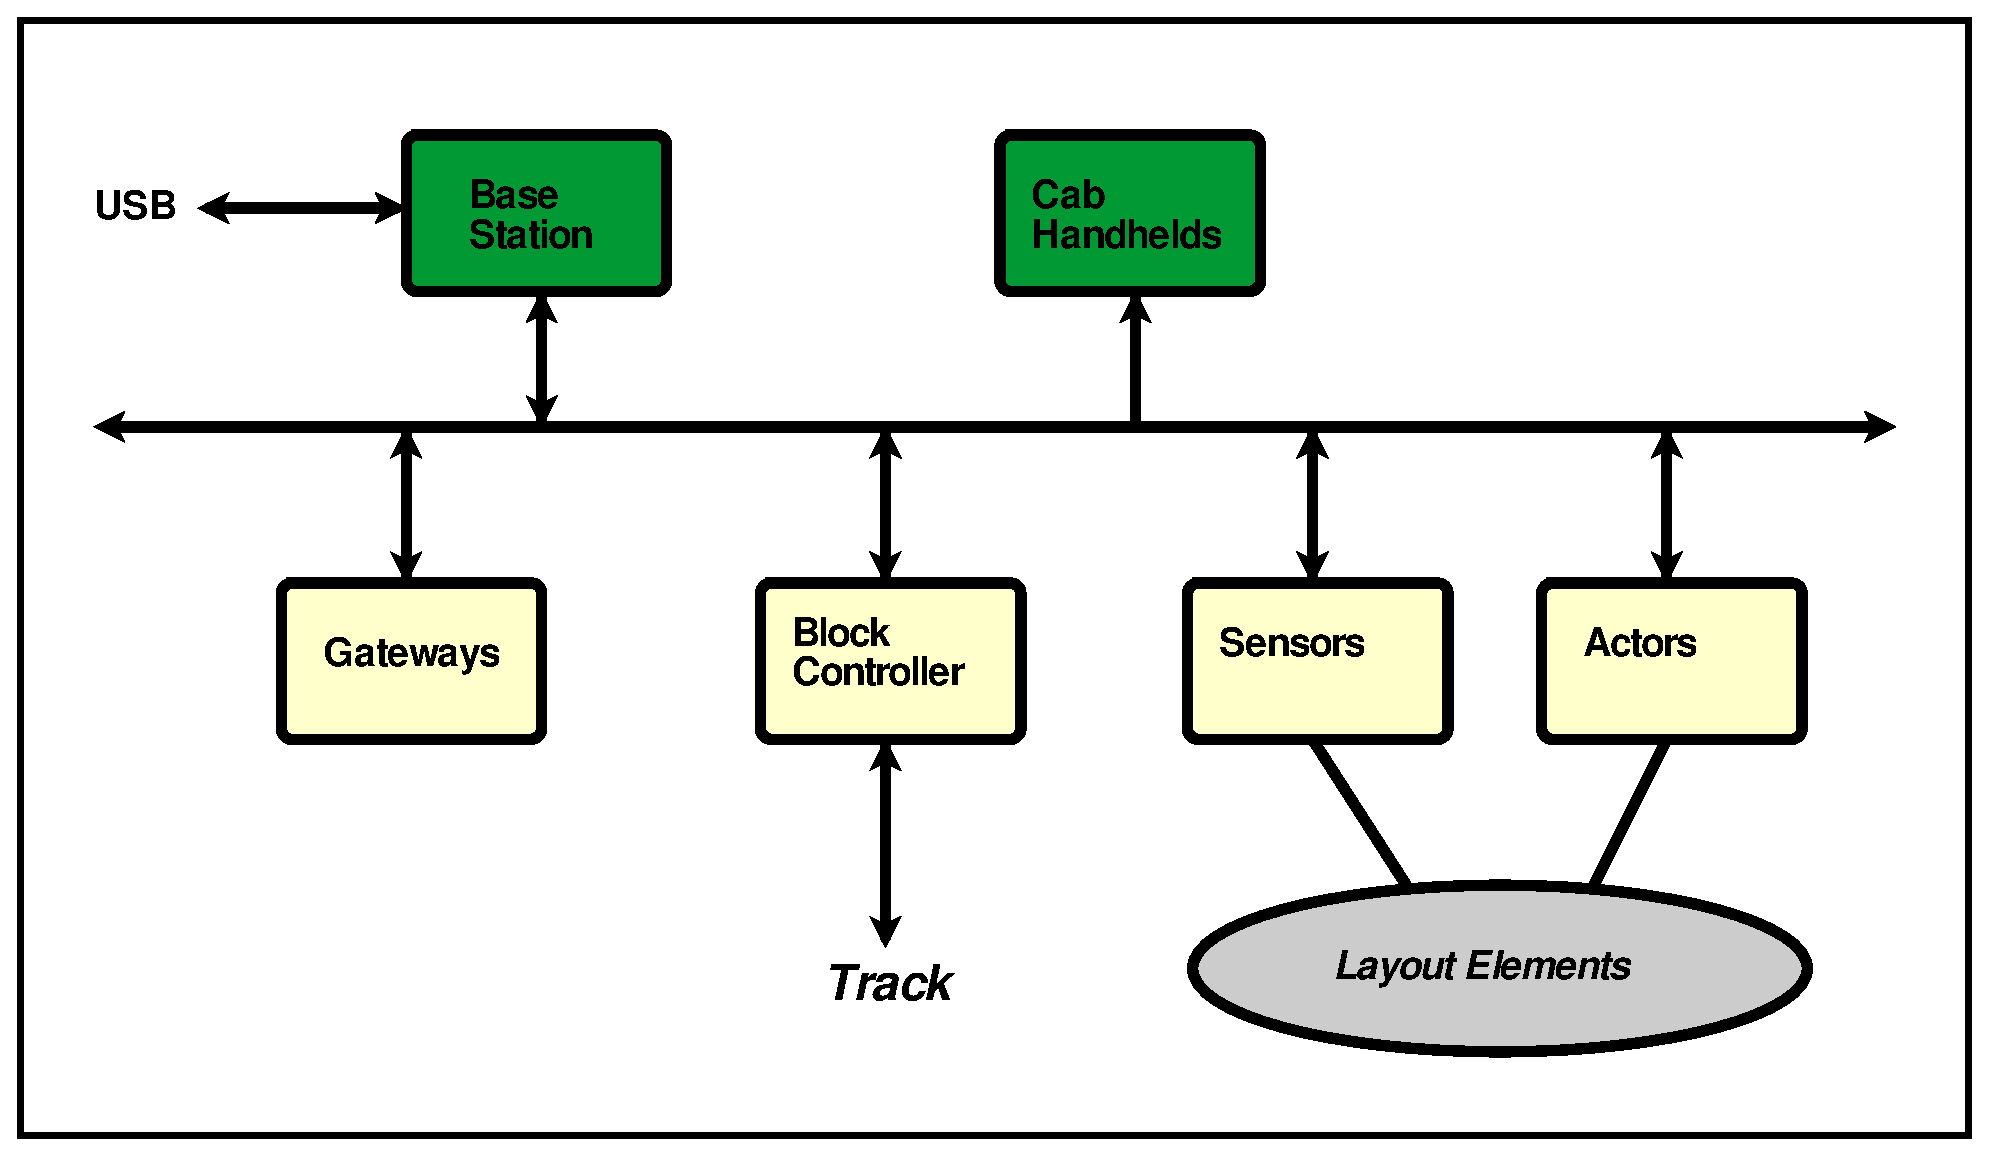
\includegraphics[page=1, width=\textwidth]{./figures/Schematic_LcsNodes-Layout-Overview.pdf}
\end{figure}

\section{Layout Control Bus}

The layout control bus is the backbone of the entire system. The current implementation is using the industry standard CAN bus. All hardware modules connect to this bus and communicate via messages. All messages are broadcasted and received by all other hardware modules on the bus. The classic CAN bus standard limits the message size to 8 bytes and this is therefore the maximum message size chosen for the LCS bus. The CAN bus also has a hardware module limit of about 110 modules for bandwidth reasons. But even for a large layout this should be sufficient. And for really large layouts, another bus system or a system with CAN bus routers, could be envisioned. The software should therefore be designed to manage thousands of connected modules. While the CAN bus technology could be exchanged, the message format and size defined as well as the broadcasting paradigm are fixed in the overall design and will not change.

\section{Hardware Module}

Everything connected to the LCS bus is a {\bf hardware module}, which is the physical entity connected to the bus. Typically it is a micro controller with the bus interface and hardware designed for the specific purpose. For example, a CAN bus interface, an AtMega Controller, and digital output drivers could form a hardware module to control railroad turnouts and signals. Base stations, handhelds and gateways are further examples of a hardware module. Hardware modules are expected to be physically located near their use and thus spread throughout the layout. Some hardware modules could be at locations that cannot be reached easily. So all interaction for configuration and operations needs to be possible through the messages on the bus. Nevertheless, putting local controls on a hardware module should not be prohibited.

A hardware module consists of a controller part and a node specific part. The controller part is the {\bf main controller}, which consists of the controller chip, a non-volatile memory to retain any data across power down, a CAN bus interface and interfaces to the node specific hardware. The node specific hardware is called the {\bf node extension}. Conceptually, both parts can be one monolithic implementation on one PCB board, but also two separate units connected by the extension connector. The are defined connectors between the boards. The hardware chapter will go into more detail on the board layouts and hardware design options.

\section{Nodes}

A hardware module is the physical implementation. A {\bf node} is the software entity running in the firmware of the hardware module. Nodes are the processing elements for the layout. Conceptually, a hardware module can host more than one node. The current implementation however supports only one node on a given hardware module. A node is uniquely identified through the {\bf node identifier}. There are two ways to set a nodeId. The first is to have central component to assign these numbers on request. The second method sets the number manually. Although a producer consumer scheme would not need a nodeId, there are many operations that are easier to configure when explicitly talking to a particular node. Both nodes and event identifiers are just numbers with no further classification scheme. A configuration system is expected to provide a classification grouping of nodes and event number ranges if needed.

A node also has a {\bf node type}, to identify what the node is capable of. Examples of nodes types are the base station, a booster, a switch module, a signal control module, and so on. While the node number is determined at startup time and can change, the node type is set via the module firmware. As the node type describes what the hardware module can do the type cannot change unless the module changes. Once the node has an assigned node number, configuration tools can configure the node via configuration messages to set the respective node variables.

A node needs to be configured and remember its configuration. For this purpose, each node contains a {\bf node map} that keeps all the information about the node, such as the number of ports, the node unique Id and so on. There is also a small set of user definable attributes to set data in a node map specific to the node. The data is stored in non-volatile memory space and on power up the node map is used to configure the node. If the module is a new module, or a module previously used in another layout, or the firmware version requires a new data layout of the node map, there is a mechanism to assign a new node number and initialize the node map with default values.

\section{Ports}

A node has a set of receiving targets, called ports. Ports connect the hardware world to the software world, and are the connection endpoints for events and actions. For example, a turnout digital signal output could be represented to the software as a port on a node. The node registers its interest in the event that target the signal. An event sent to the node and port combination then triggers a callback to the node firmware to handle the incoming events. Although a node can broadcast an event anytime by just sending the corresponding message, the event to send is typically associated with an outbound port for configuration purposes. In addition to the event immediate processing, the event handling can be associated with a timer delay value. On event reception the timer value will delay the event callback invocation or broadcast.

A node has a {\bf port map} that contains one entry for each defined port. {\bf port map entries} describe the configuration attributes and state of the port such as the port type. There is also a small set of user definable attributes to set data in a port map entry specific to the port. These attributes can be used by the firmware programmer to store port specific data items such as a hardware pin or a limit value in the port map.

\section{Attributes}

{\bf Node attributes} and {\bf port attributes} are conceptually similar to the CV resources in a DCC decoder. Many decoders, including the DCC subsystem decoders, feature a set of variables that can be queried or set. The LCS layout system implements a slightly different scheme based on items. In contrast to a purely decoder variable scheme an item can also just represent just an action such as setting an output signal. Items are passed parameter data to further qualify the item. Items are just numbers assigned. The range of item numbers is divided into a reserved section for the layout system itself, and a user defined range that allows for a great flexibility to implement the functions on a particular node and port. The meaning of user defined items is entirely up to the firmware programmer. If it is desired to have a variables, a combination of items and attributes can provide the traditional scheme as well. In addition, there are node local variables, called attributes, available to the firmware programmer for storing data items.

\section{Events}

The LCS message bus, hardware module, node and ports describe layout and are statically configured. For nodes to interact, {\bf events} and their configuration is necessary. An event is a message that a node will broadcast via the bus. Every other node on this bus will receive the event and if interested act on the event. The sender is the producer, the receiver is the consumer. Many producers can produce the same event, many consumers can act on the same event. The {\bf event Id}, a 16 bit number, is unique across the layout and assigned by a configuration tool during the configuration process. Other than being unique, there is no special meaning, the number is arbitrary. There are in total 65536 events available.

In addition to the event Id, an event message contains the node Id of the sender. While most events will be an ON/OFF event, events can also have additional data. For example an overload event sent by a booster node, could send the actual current consumption value in the event message. A consumer node registers its interest in an event by being configured to react to this event on a specific port. The node maintains an {\bf event map}, which contains one entry for each event id / port id combination. For the eventing system to work, the nodeID is not required. Any port on any node can react to an event, any node can broadcast an event.

To connect producers to consumers, both parties need to be told what to do with a defined event. A producer node outbound port needs to be told what event to send for a given sensor observation. For example, a simple front panel push button needs to be told what event to send when pushed. Likewise, a consumer node inbound port needs to be told what events it is interested in and what the port should do when this event is received. Both meet through the event number used. While an inbound port can be configured to listen to many event Ids, an outbound port will exactly broadcast one eventId.

Any port on any node can react to an event, any node can broadcast an event. Still, addressing a node and port combination explicitly is required for two reasons. The first is of course the configuration of the node and port attributes. Configuration data needs to go directly to the specified node and port. The second reason is for directly accessing a resource on the layout. For example, directly setting a turnout connected to one node. While this could also be implemented with associated an event to send when operating a turnout, it has shown beneficial and easier to configure also directly access such a resource through a dedicated node/port address.

\section{DCC Subsystem}

The node, ports and events are the foundation for building a layout system based on the producer / consumer scheme. The scheme will be used heavily for implementing turnout control, signals, signal blocks and so on. In addition, there is the management of the mobile equipment, i.e. locomotives. The DCC subsystem is the other big part of our layout control system. In a sense it is another bus represented by the track sections.

LCS messages for DCC commands are broadcasted from controlling devices. For example, a handheld broadcasts a speed setting DCC command. In a layout there is one base station node which is responsible to produce the DCC signals for the track. The DCC signals are part of the physical LCS bus. While a base station design could directly supply the signal current to the track, larger layouts will typically have one or more boosters. They take the DCC signal from the LCS bus lines and generate the DCC signal current for their track section. All LCS messages for DCC operations are broadcasting messages, all nodes can send them, all nodes can receive them. Handhelds, base station and boosters are thus just nodes on the LCS bus. Only the base station will however generate the DCC signal.

The DCC standard defines mobile and stationary decoders. The DCC signal could also be used to control for example a set of turnouts via a stationary decoder. The LCS DCC  message set contains messages for addressing a stationary decoder. Since the commands for stationary equipment are just DCC commands, they will be transmitted via the track as well and take away bandwidth on the track. A layout will therefore more likely use the LCS bus for implementing the management of stationary equipment. Besides, the producer / consumer model allows for a much greater flexibility when building larger and partially automated layouts.

\section{Analog Subsystem}

The layout control system is primarily a digital control system. There are however layout use cases where there are many analog locomotives that would represent a significant investment when converting to DCC or that cannot easily be equipped with a DCC decoder. In a DCC subsystem the decoder is in the locomotive and many locomotives can run therefore on the same track. In an analog system, the locomotive has no capabilities and therefore the track needs to be divided into sections that can be controlled individually. One locomotive per section is the condition. In a sense the decoder becomes part of the track section. The layout control system offers support for building such a track section subsystem. Often the sections are combined into blocks and build the foundation for a block signaling system. Note that the rest of the layout control system is of course digital. What is typically the booster to support a section of track, is the block controller for an analog layout. We will see in the later chapters that booster and block controller are very similar and design a block controller to accommodate both use cases.

\section{Configuration Mode}

Before operations the nodes, ports and events need to be configured. Once a node has an assigned valid nodeId, the node configuration is the process of configuring a node global information, the event map information and the finally the port information. The information is backed by non-volatile storage, such that there is a consistent state upon node power up. During operations, these value can of course change, but are always reset to the initial value upon startup.

The primary process of configuration is inventing events numbers and assigning them producers and consumers. The process follows the general "if this then that" principle. On the producer side the configuration process assigns a port to an event, i.e. the push of a button to an event to send. If this button is pushed then send that event. On the consumer side the configuration process is to assign the event to a port. If this event is received then execute that port action.

After the node is up and running with a valid node Id, there are event configuration messages than can be send to the node to set the event mapping table with this information. The event map table is the mapping between the event and the port associated. Events are thus configured by "teaching" the target node what port to inform about an occurring event.

\section{Operation Mode}

Besides the basic producer/consumer model with the event messages as communication mechanism, there are several LCS control and info messages used for managing the overall layout with signals turnouts and so on as well as the physical track and the running equipment. In a layout, the track typically consist of one or more sections, each managed by a booster or block controller node. Track sections are monitored for their power consumption to detect short circuits. Back communication channels such as RailCom are handled by the booster node and provide information about the running equipment. Stationary equipment such as turnouts and signals as well as detectors, such as track occupancy detectors or turnout setting detectors are monitored and controlled through LCS messages and the event system. Conceptually any node can send and receive such event, info or control messages. Some nodes, however have a special role.

For example, the key module for layout operations is the {\bf base station}. The base station, a node itself, is primarily responsible for managing the active locomotives on the layout. When a control handheld wants to run a locomotive, a cab session for that locomotive is established by the base station. Within the session, the locomotive speed, direction and functions are controlled through the cab handheld sending the respective messages. The base station is responsible for generating the DCC packets that are sent by the booster or block controller power module to the actual track sections. Booster and block controller module are - you guessed it - node themselves.

Finally, there are LCS nodes that represent cab handhelds to control a locomotive or consists, layout panel connectors, gateways to other layout protocols, sensors and actors to implement for example turnout control, signaling, section occupancy detections and many more. All these components share the common LCS bus and use ports and events to implement the capabilities for operating a layout.

In a layout with many track sections the {\bf block controller} is a special node that will manage a block on the layout. Like all other nodes, a block controller itself is a node that can react to events and is controller and monitored by LCS messages. There will be several chapters devoted to this topic later.

\section{Summary}

This chapter introduced the basic concepts of the layout control system described in this book. It follows very few overall guiding principles. Above all, there is the clear separation of what needs to be available for operating the mobile equipments, i.e. locomotives, and the stationary layout elements. Controlling mobile decoders are left to the DCC subsystem, all other communication takes place via the LCS bus, which is the bus to which all of the hardware modules connect. Hardware modules host the nodes. Currently, a hardware module hosts exactly one node. A node can contains one or many ports, which are the endpoints for the event system. There is a set of user allocated attributes available to node and ports. Node, port and attribute data are backed by non-volatile memory, so that a restart will use defined initial values. Nodes and their ports are also directly addressable, which is needed for configuration purposes and the directly addressable components model. Using the producer / consumer paradigm, sensors generate events and interested actors just act on them. The configuration process is simply to assign the same event to the producer node and consumer node / port id when they should work together.

The communication bus should rest on a reliable bus with a sufficient bandwidth. Although the CAN bus is used in the initial implementation, it is just one option and other technologies can be considered. In all cases however, the message format should be available for a variety of bus technologies. Our messages are therefore short, up to eight data bytes. This causes on the one hand some complexity for data items larger than a few bytes on the other hand no messages blocks the bus for a longer period. The bus technology is expected to reliably deliver a message but does not ensure its processing. This must be ensured through a request reply message scheme built on top.


    \chapter{Message Formats}

Before diving into the actual design of the software and hardware components, let us first outline the message data formats as they flow on the layout control bus. It is the foundation of the layout control system, so let's have a first brief look at all the messages defined. This chapter will provide the overview on the available messages and give a short introduction to what they do. Later chapters build on it and explain how the messages are used for designing LCS node functions. The layout control system messages can be grouped into several categories:

\begin{itemize}
    \item General management
    \item Node and Port management
    \item Event management
    \item DCC Track management
    \item DCC Locomotive Decoder management
    \item DCC Accessory Decoder management
    \item RailCom DCC Packet management
    \item Raw DCC Packet management
\end{itemize}

All nodes communicate via the layout control bus by broadcasting messages. Every node can send a message, and every node receives the message broadcasted. There is no central master. The current implementation is using the CAN bus, which ensures by definition that a message is correctly transmitted. However, it does not guarantee that the receiver actually processed the message. For critical messages, a request-reply scheme is implemented on top. Also, to address possible bus congestion, a priority scheme for messages is implemented to ensure that each message has a chance for being transmitted.

\section{LCS Message Format}

A message is a data packet of up to 8 bytes. The first byte represents the operation code. It encodes the length of the entire packet and opcode number. The first 3 bits represent the length of the message, the remaining 5 bits represent the opCode. For a given message length, there are 32 possible opcode numbers. The last opcode number in each group, 0x1F, is reserved for possible extensions of the opcode number range. The remaining bytes are the data bytes, and there can be zero to seven bytes. The message format is independent of the underlying transport method. If the bus technology were replaced, the payload would still be the same. For example, an Ethernet gateway could send those messages via the UDP protocol. The messages often contain 16-bit values. They are stored in two bytes, the most significant byte first and labeled ``xxx-H'' in the message descriptions to come. The message format shown in the tables of this chapter just presents the opCode mnemonic. The actual value can be found in the core library include file.

\section{General Management}

The general management message group contains commands for dealing with the layout system itself. The reset command \texttt{(RESET)} directs all hardware modules, a node, or a port on a node to perform a reset. The entire bus itself can be turned on and off \texttt{(BUS-ON, BUS-OFF)}, enabling or suppressing the message flow. Once the bus is off, all nodes wait for the bus to be turned on again. Finally, there are messages for pinging a node \texttt{(PING)} and request acknowledgement \texttt{(ACK/ERR)}.

\begin{table}[h!]
    \begin{center}
        \caption{General Management}
        \begin{tabular}{|l|l|l|l|l|l|l|l|}
            \toprule
            \textbf{Opcode} & \textbf{Data1} & \textbf{Data2} & \textbf{Data3} & \textbf{Data4} & \textbf{Data5} & \textbf{Data6} & \textbf{Data7} \\
            \midrule
            RESET & npId-H & npId-L & flags & & & & \\
            BUS-ON & & & & & & & \\
            BUS-OFF & & & & & & & \\
            SYS-TIME & arg1 & arg2 & arg3 & arg4 & & & \\
            LCS-INFO & arg1 & arg2 & arg3 & arg4 & & & \\
            PING & npId-H & npId-L & & & & & \\
            ACK & npId-H & npId-L & & & & & \\
            ERR & npId-H & npId-L & code & arg1 & arg2 & & \\
            \bottomrule
        \end{tabular}
    \end{center}
\end{table}

\subsection*{Additional Notes}
\begin{itemize}
    \item Do we need a message for a central system time concept?
    \item Do we need a message for a message that describes the global LCS capabilities?
    \item Do we need an emergency stop message that every node can emit?
\end{itemize}

\section{Node and Port Management}

When a hardware module is powered on, the first task is to establish the node Id in order to broadcast and receive messages. The \texttt{(REQ-NID)} and \texttt{(REP-ID)} messages are the messages used to implement the protocol for establishing the nodeId. More on this in the chapter on message protocols. A virgin node has the hardware module-specific node type and a node Id of \texttt{NIL} also be set directly through the \texttt{(SET-NID)} command. This is typically done by a configuration tool.

\begin{table}[ht!]
    \begin{center}
        \caption{Node and Port Management}
        \begin{tabular}{|l|l|l|l|l|l|l|l|}
            \toprule
            \textbf{Opcode} & \textbf{Data1} & \textbf{Data2} & \textbf{Data3} & \textbf{Data4} & \textbf{Data5} & \textbf{Data6} & \textbf{Data7} \\
            \midrule
            REQ-NID & nId-H & nId-L & nUID-4 & nUID-3 & nUID-2 & nUID-1 & flags \\
            REP-NID & nId-H & nId-L & nUID-4 & nUID-3 & nUID-2 & nUID-1 & flags \\
            SET-NID & nId-H & nId-L & nUID-4 & nUID-3 & nUID-2 & nUID-1 & flags \\
            NCOL    & nId-H & nId-L & nUID-4 & nUID-3 & nUID-2 & nUID-1 & \\
            \bottomrule
        \end{tabular}
    \end{center}
\end{table}


All nodes monitor the message flow to detect a potential node collision. This could be for example the case when a node from one layout is installed in another layout. When a node detects a collision, it will broadcast the \texttt{(NCOL)} message and enter a halt state. Manual interaction is required. A node can be restarted with the \texttt{(RES-NODE)} command, given that it still reacts to messages on the bus. All ports on the node will also be initialized. In addition a specific port on a node can be initialized. The hardware module replies with an \texttt{(ACK)} message for a successful node Id and completes the node Id allocation process. As the messages hows, node and port ID are combined. LCS can accommodate up to 4095 nodes, each of which can host up to 15 ports. A Node ID 0 is the NIL node. Depending on the context, a port Id of zero refers all ports on the node or just the node itself.

The query node \texttt{(NODE-GET)} and node reply messages \texttt{(NODE-REP)} are available to obtain attribute data from the node or port. The \texttt{(NODE-SET)} allows to set attributes for a node or port for the targeted node. Items are numbers assigned to a data location or an activity. There are reserved items such as getting the number of ports, or setting an LED. In addition, the firmware programmer can also define items with node specific meaning. The firmware programmer defined items are accessible via the \texttt{(NODE-REQ)} and \texttt{(NODE-REP)} messages.

\begin{table}[ht!]
    \begin{center}
        \caption{Node and Port Management}
        \begin{tabular}{|l|l|l|l|l|l|l|l|}
            \toprule
            \textbf{Opcode} & \textbf{Data1} & \textbf{Data2} & \textbf{Data3} & \textbf{Data4} & \textbf{Data5} & \textbf{Data6} & \textbf{Data7} \\
            \midrule
            NODE-GET & npId-H & npId-L & item & arg1-H & arg1-L & arg2-H & arg2-L \\
            NODE-PUT & npId-H & npId-L & item & val1-H & val1-L & val2-H & val2-L \\
            NODE-REQ & npId-H & npId-L & item & arg1-H & arg1-L & arg2-H & arg2-L \\
            NODE-REP & npId-H & npId-L & item & arg1-H & arg1-L & arg2-H & arg2-L \\
            \bottomrule
        \end{tabular}
    \end{center}
\end{table}

Nodes do not react to attribute and user defined request messages when in operations mode. To configure a node, the node needs to be put into configuration mode. The \texttt{(OPS)} and \texttt{(CFG)} commands are used to put a node into configuration mode or operation mode. Not all messages are supported in operations mode and vice versa. For example, to set a new nodeId, the node first needs to be put in configuration mode. During configuration mode, no operational messages are processed.

\begin{table}[ht!]
    \begin{center}
        \caption{Node and Port Management}
        \begin{tabular}{|l|l|l|l|l|l|l|l|}
            \toprule
            \textbf{Opcode} & \textbf{Data1} & \textbf{Data2} & \textbf{Data3} & \textbf{Data4} & \textbf{Data5} & \textbf{Data6} & \textbf{Data7} \\
            \midrule
            OPS & npId-H & npId-L & & & & & \\
            CFG & npId-H & npId-L & & & & & \\
            \bottomrule
        \end{tabular}
    \end{center}
\end{table}


\section{Event Management}

The event management group contains the messages to configure the node event map and messages to broadcast an event and messages to read out event data. The (SET-NODE) with the item value to set and remove an event map entry from the event map is used to manage the event map. An inbound port can register for many events to listen to, and an outbound port will have exactly one event to broadcast. Ports and Events are numbered from 1 onward. When configuring, the portId \texttt{NIL} has a special meaning in that it refers to all portIds on the node.

\begin{table}[ht!]
    \begin{center}
        \caption{Event Management}
        \begin{tabular}{|l|l|l|l|l|l|l|l|}
            \toprule
            \textbf{Opcode} & \textbf{Data1} & \textbf{Data2} & \textbf{Data3} & \textbf{Data4} & \textbf{Data5} & \textbf{Data6} & \textbf{Data7} \\
            \midrule
            EVT-ON & npId-H & npId-L & evId-H & evId-L & & & \\
            EVT-OFF & npId-H & npId-L & evId-H & evId-L & & & \\
            EVT & npId-H & npId-L & evId-H & evId-L & arg-H & arg-L & \\
            \bottomrule
        \end{tabular}
    \end{center}
\end{table}

\section{DCC Track Management}

Model railroads run on tracks. Imagine that. While on a smaller layout, there is just the track, the track on a larger layout is typically divided into several sections, each controlled by a track node \textnormal{(centralized node or decentralized port)}. The system allows to report back the track sections status \textnormal{(in terms of occupied, free, and detecting the number of engines currently present)}. These messages allow the control of turnouts and monitoring of sections' status.

\begin{table}[ht!]
    \begin{center}
        \caption{DCC Track Management}
        \begin{tabular}{|l|l|l|l|l|l|l|l|}
            \toprule
            \textbf{Opcode} & \textbf{Data1} & \textbf{Data2} & \textbf{Data3} & \textbf{Data4} & \textbf{Data5} & \textbf{Data6} & \textbf{Data7} \\
            \midrule
            TON & npId-H & npId-L & & & & & \\
            TOF & npId-H & npId-L & & & & & \\
            \bottomrule
        \end{tabular}
    \end{center}
\end{table}

\section{DCC Locomotive Decoder Management}

Locomotive management comprises the set of messages that the base station uses to control the running equipment. To control a locomotive, a session needs to be established \texttt{(REQ-LOC)}. This command is typically sent by a cab handheld and handled by the base station. The base station allocates a session and replies with the \texttt{(REP-LOC)} message that contains the initial settings for the locomotive speed and direction. \text{(REL-LOC)} closes a previously allocated session. The base station answers with the \texttt{(REP-LOC)} message. The data for an existing DCC session can requested with the \texttt{(QRY-LOC)} command. Data about a locomotive in a consist is obtained with the \texttt{(QRY-LCON)} command. In both cases the base station answers with the \texttt{(REP-LOC)} message.

\begin{table}[ht!]
    \begin{center}
        \caption{DCC Locomotive Decoder Management}
        \begin{tabular}{|l|l|l|l|l|l|l|l|}
            \toprule
            \textbf{Opcode} & \textbf{Data1} & \textbf{Data2} & \textbf{Data3} & \textbf{Data4} & \textbf{Data5} & \textbf{Data6} & \textbf{Data7} \\
            \midrule
            REQ-LOC & adr-H & adr-L & flags & & & & \\
            REP-LOC & sId & adr-H & adr-L & spDir & fn1 & fn2 & fn3 \\
            REL-LOC & sId & & & & & & \\
            QRY-LOC & sId & & & & & & \\
            QRY-LCON & conId & index & & & & & \\
            \bottomrule
        \end{tabular}
    \end{center}
\end{table}

Once the locomotive session is established, the \texttt{(SET-LSPD)}, \texttt{(SET-LMOD)}, \texttt{(SET-LFON)}, \texttt{(SET-LOF)} and \texttt{(SET-FGRP)} are the commands sent by a cab handheld and executed by the base station to control the locomotive speed, direction and functions. \texttt{(SET-LCON)} deals with the locomotive consist management and \texttt{(KEEP)} is sent periodically to indicate that the session is still alive. The locomotive session management is explained in more detail in a later chapter when we talk about the base station.

\begin{table}[ht!]
    \begin{center}
        \caption{DCC Locomotive Decoder Management}
        \begin{tabular}{|l|l|l|l|l|l|l|l|}
            \toprule
            \textbf{Opcode} & \textbf{Data1} & \textbf{Data2} & \textbf{Data3} & \textbf{Data4} & \textbf{Data5} & \textbf{Data6} & \textbf{Data7} \\
            \midrule
            SET-LSPD & sId & spDir & & & & & \\
            SET-LMOD & sId & flags & & & & & \\
            SET-LFON & sId & fNum  & & & & & \\
            SET-LFOF & sId & fNum  & & & & & \\
            SET-FGRP & sId & fGrp  & data & & & & \\
            SET-LCON & sId & conId & flags & & & & \\
            KEEP & sId & & & & & & \\
            \bottomrule
        \end{tabular}
    \end{center}
\end{table}

Locomotive decoders contain configuration variables too. They are called CV variables. The base station node supports the decoder CV programming on a dedicated track with the \texttt{(REQ-CVS)}, \texttt{(REP-CVS)} and \texttt{(SET-CVS)} messages. The \texttt{(SET-CVM)} message supports setting a CV while the engine is on the main track. \texttt{(DCC-ERR)} is returned when an invalid operation is detected.

\begin{table}[ht!]
    \begin{center}
        \caption{DCC Locomotive Decoder Management}
        \begin{tabular}{|l|l|l|l|l|l|l|l|}
            \toprule
            \textbf{Opcode} & \textbf{Data1} & \textbf{Data2} & \textbf{Data3} & \textbf{Data4} & \textbf{Data5} & \textbf{Data6} & \textbf{Data7} \\
            \midrule
            SET-LSPD & sId & cv-H & cv-L & mode & val & & \\
            REQ-CVS  & cv-H & cv-L & mode & val & & & \\
            REP-CVS  & cv-H & cv-L & val  & & & & \\
            SET-CVS  & cv-H & cv-L & mode & val & & & \\
            \bottomrule
        \end{tabular}
    \end{center}
\end{table}

The SET-CVM command allows to write to a decoder CV while the decoder is on the main track. Without the RailCom channel, CVs can be set but there is not way to validate that the operation was successful.

\section{DCC Accessory Decoder Management}

Besides locomotives, the DCC standards defines stationary decoders, called accessories. An example is a decoder for setting a turnout or signal. There is a basic and an extended format. The \texttt{(SET-BACC)} and \texttt{(SET-EACC)} command will send the DCC packets for stationary decoders. Similar to the mobile decoders, there are POM / XPOM messages to access the stationary decoder via RailCom capabilities.

\begin{table}[ht!]
    \begin{center}
        \caption{DCC Accessory Decoder Management}
        \begin{tabular}{|l|l|l|l|l|l|l|l|}
            \toprule
            \textbf{Opcode} & \textbf{Data1} & \textbf{Data2} & \textbf{Data3} & \textbf{Data4} & \textbf{Data5} & \textbf{Data6} & \textbf{Data7} \\
            \midrule
            SET-BACC & adr-H & adr-L & flags & & & & \\
            SET-EACC & adr-H & adr-L & val & & & & \\
            \bottomrule
        \end{tabular}
    \end{center}
\end{table}

These commands are there for completeness of the DCC control interfaces. There could be devices that are connected via the DCC track that we need to support. However, in a layout control system the setting of turnouts, signals and other accessory devices are more likely handled via the layout control bus messages and not via DCC packets to the track. This way, there is more bandwidth for locomotive decoder DCC packets.

\section{RailCom DCC Packet management}

With the introduction of the RailCom communication channel, the decoder can also send data back to a base station. The DCC POM and XPOM packets can now not only write data but also read out decoder data via the RailCom back channel. The following messages allow to send the POM / XPOM DCC packets and get their RailCom based replies.

\begin{table}[ht!]
    \begin{center}
        \caption{RailCom DCC Packet management}
        \begin{tabular}{|l|l|l|l|l|l|l|l|}
            \toprule
            \textbf{Opcode}  & \textbf{Data1} & \textbf{Data2} & \textbf{Data3} & \textbf{Data4} & \textbf{Data5} & \textbf{Data6} & \textbf{Data7} \\
            \midrule
            SET-MPOM & sId & ctrl & arg1 & arg2 & arg3 & arg4 & \\
            REQ-MPOM & sId & ctrl & arg1 & arg2 & arg3 & arg4 & \\
            REP-MPOM & sId & ctrl & arg1 & arg2 & arg3 & arg4 & \\
            SET-APOM & adr-H & adr-L & ctrl & arg1 & arg2 & arg3 & arg4 \\
            REQ-APOM & adr-H & adr-L & ctrl & arg1 & arg2 & arg3 & arg4 \\
            REP-APOM & adr-H & adr-L & ctrl & arg1 & arg2 & arg3 & arg4 \\
            \bottomrule
        \end{tabular}
    \end{center}
\end{table}

The XPOM messages are DCC messages that are larger than what a CAN bus packet can hold. With the introduction of DCC-A such a packet can hold up to 15 bytes. The LCS messages therefore are sent in chunks with a frame sequence number and it is the responsibility of the receiving node to combine the chunks to the larger DCC packet.

\section{Raw DCC Packet Management}

The base station allows to send raw DCC packets to the track. The \texttt{(SEND-DCC3)}, \texttt{(SEND-DCC4)}, \texttt{(SEND-DCC5)} and \texttt{(SEND-DCC6)} are the messages to send these packets. Any node can broadcast such a message, the base station is the target for these messages and will just send them without further checking. So you better put the DCC standard document under your pillow.

\begin{table}[ht!]
    \begin{center}
        \caption{RRaw DCC Packet Management}
        \begin{tabular}{|l|l|l|l|l|l|l|l|}
            \toprule
            \textbf{Opcode}  & \textbf{Data1} & \textbf{Data2} & \textbf{Data3} & \textbf{Data4} & \textbf{Data5} & \textbf{Data6} & \textbf{Data7} \\
            \midrule
            SEND-DCC3 & arg1 & arg2 & arg3 & & & & \\
            SEND-DCC4 & arg1 & arg2 & arg3 & arg4 & & & \\
            SEND-DCC5 & arg1 & arg2 & arg3 & arg4 & arg5 & & \\
            SEND-DCC6 & arg1 & arg2 & arg3 & arg4 & arg5 & arg6 & \\
            \bottomrule
        \end{tabular}
    \end{center}
\end{table}

The above messages can send a packet with up to six bytes. With the evolving DCC standard, larger messages have been defined. The XPOM DCC messages are a good example. To send such a large DCC packet, it is decomposed into up to four LCS messages. The base station will assemble the DCC packet and then send it. 

\begin{table}[ht!]
    \begin{center}
        \caption{RRaw DCC Packet Management}
        \begin{tabular}{|l|l|l|l|l|l|l|l|}
            \toprule
            \textbf{Opcode}  & \textbf{Data1} & \textbf{Data2} & \textbf{Data3} & \textbf{Data4} & \textbf{Data5} & \textbf{Data6} & \textbf{Data7} \\
            \midrule
            SEND-DCCM & ctrl & arg1 & arg2 & arg3 & arg4 & & \\
            \bottomrule
        \end{tabular}
    \end{center}
\end{table}

\section{DCC errors and status}

Some DCC commands return an acknowledgment or an error for the outcome of a DCC subsystem request. The \texttt{(DCC-ACK)} and \texttt{(DCC-ERR)} messages are defined for this purpose.

\begin{table}[ht!]
    \begin{center}
        \caption{RRaw DCC Packet Management}
        \begin{tabular}{|l|l|l|l|l|l|l|l|}
            \toprule
            \textbf{Opcode}  & \textbf{Data1} & \textbf{Data2} & \textbf{Data3} & \textbf{Data4} & \textbf{Data5} & \textbf{Data6} & \textbf{Data7} \\
            \midrule
            DCC-ACK & & & & & & & \\
            DCC-ERR & code & arg1 & arg2 & & & & \\
            \bottomrule
        \end{tabular}
    \end{center}
\end{table}

\section{Analog Engines}

The messages defined for the DCC locomotive session management as outlined above are also used for the analog engines. An analog engine will just like its digital counterpart have an allocated locomotive session and the speed/dir command is supported. All other commands will of course not be applicable. The speed/dir command will be sent out on the bus and whoever is in control of the track section where the analog engine is supposed to be, will manage that locomotive. In the following chapters we will answer the question of how exactly multiple analog engines can run on a layout.

\section{Summary}

The layout system is a system of nodes that talk to each other. At the heart are consequently messages. The message format is built upon an 8-byte message format that is suitable for the industry standard CAN bus. Although there are many other standards and communication protocols, the CAN bus is a widely used bus. Since all data is encoded in the message, there is no reason to select another communication media. But right now, it is CAN.



    %-------------------------------------------------------------------------------------------------------
%-------------------------------------------------------------------------------------------------------
\chapter{Message Protocols}

This chapter will present how the messages presented in the previous chapter are used to form the protocols for layout configuration and operations. We begin with node management and port management. Next, the event system is described. Finally, the DCC locomotive and track management related commands and messages round up this chapter. The protocols are described as a set of high level messages flow from requestor to receiver and back.

\section{Node startup}

Node startup includes all the software steps to initialize local data structures, hardware components and whatever else the hardware module requires. To the layout system, the node needs to be uniquely identified across the layout. A configuration software will use the nodeId to manage the node. The \texttt{(REQ-NID)} and \texttt{(REP-NID)} messages are used to establish the nodeId on node startup. On startup the current nodeId stored in the module non-volatile memory is broadcasted. The \texttt{(REQ-NID)} message also contains the node UID. This unique identifier is created when the node is first initialized and all non-volatile data structures are built. The UID will not change until the node is explicitly re-initialized again.

After sending the \texttt{(REQ-NID)} message the node awaits the reply \texttt{(REP-NID)}. The reply typically comes from a base station node or configuration software. In fact, any node can take on the role of assigning nodeIds. But a layout can only have one such node in charge of assigning nodeIds. The reply message contains the UID and the nodeId assigned. For a brand new module, this is will the node nodeId from now on.

\begin{table}[ht!]
    \centering
    \caption{Node startup}
    \begin{tabular}{|p{0.42\textwidth}|p{0.42\textwidth}|}
        \toprule
        \textbf{node} & \textbf{base Station} \\
        \midrule
        REQ-NID (nodeId, nodeUID) \texttt{->} & \\
        & \texttt{<-} REP-NID (nodeId, nodeUID) or timeout \\
        \bottomrule
    \end{tabular}
\end{table}

The nodeUID plays an important role to detect nodeId conflicts. If there are two modules with the same nodeId, the nodeUID is still different. A requesting node will check the \texttt{(REP-NID)} answer, comparing the nodeUID in the message to its own nodeUID. If the UID matches, the nodeId in the message will be the nodeId to set. Note that it can be the one already used, or a new nodeId. If the UIDs do not match, we have two nodes assigned the same nodeId. Both nodes will enter the collision and await manual resolution.

The above nodeId setup scheme requires the presence of a central node, such a base station, to validate and assign node identifiers. In addition, the nodeId can also be assigned by the firmware programmer and passed to the library setup routine. Once assigned, the node is accessible and the node number can be changed anytime later with the \texttt{(SET-NID)} command. All nodes are always able to detect a nodeId conflict. If two or more nodes have the same nodeId, each node will send an \texttt{(NCOL)} message and go into halted state, repeating the collision message. Manual intervention is required to resolve the conflict through explicitly assigning a new nodeId.

\section{Switching between Modes}

After node startup, a node normally enters the operation state. During configuration, certain commands are available and conversely some operational commands are disabled. A node is put into the respective mode with the \texttt{(CFG)} and \texttt{(OPS)} message command.

\begin{table}[ht!]
    \begin{center}
        \caption{Switching between Configuration and Operations mode}
        \begin{tabular}{|p{0.42\textwidth} c p{0.42\textwidth}|}
            \toprule
            \textbf{base Station} & & \textbf{target node} \\
            \midrule
            CFG/OPS & \texttt{->} & \\
            & \texttt{<-} & ACK/ERR ( nodeId ) or timeout \\
            \bottomrule
        \end{tabular}
    \end{center}
\end{table}

\section{Setting a new Node Id}

A configuration tool can also set the node Id to a new value. This can only be done when the node is configuration mode. The following sequence of messages shows how the node is temporarily put into configuration mode for setting a new node Id.

\begin{table}[ht!]
    \begin{center}
        \caption{Switching between Configuration and Operations mode}
        \begin{tabular}{|p{0.42\textwidth} c p{0.42\textwidth}|}
            \toprule
            \textbf{Base Station} & & \textbf{Node} \\
            \midrule
            \text{CFG ( nodeId )} & \texttt{->}  & node enters config mode \\
            & \texttt{<-} & ACK/ERR ( nodeId ) or timeout \\
            \midrule
            \text{SET-NID ( nodeId, nodeUID )} \texttt{->}  & &  \\
            & \texttt{<-} & ACK/ERR ( nodeId ) or timeout \\
            \midrule
            \text{OPS ( nodeId )} & \texttt{->}  & node enters operations mode \\
            & \texttt{<-} & ACK/ERR ( nodeId ) or timeout \\
            \bottomrule
        \end{tabular}
    \end{center}
\end{table}

It is important to note that the assignment of a node Id through a configuration tool will not result in a potential node Id conflict resolution or detection. This is the responsibility of the configuration tool when using this command. The node Id, once assigned on one way or another, is the handle to address the node. There is of course an interest to not change these numbers every time a new hardware module is added to the layout.

\section{Node Ping}

Any node can ping any other node. The target node responds with an (ACK) message. If the nodeId is NIL, all nodes are requested to send an acknowledge (ACK). This command can be used to enumerate which nodes are out there. However, the receiver has to be able to handle the flood of (ACK) messages coming in.

\begin{table}[ht!]
    \begin{center}
        \caption{Node ping}
        \begin{tabular}{|p{0.42\textwidth} c p{0.42\textwidth}|}
            \toprule
            \textbf{requesting node} & & \textbf{ target node} \\
            \midrule
            PING & \texttt{->} & \\
            \midrule
            & \texttt{<-} & ACK ( nodeId ) or timeout \\
            \bottomrule
        \end{tabular}
    \end{center}
\end{table}

\section{Node and Port Reset}

A node or individual port can be restarted. This command can be used in configuration as well as operations mode. The node or will perform a restart and initialize its state from the non-volatile memory. A port ID of zero will reset the node and all the ports on the node.

\begin{table}[ht!]
    \begin{center}
        \caption{Node and Port Reset}
        \begin{tabular}{|p{0.42\textwidth} c p{0.42\textwidth}|}
            \toprule
            \textbf{requesting node} & & \textbf{ target node} \\
            \midrule
            RES-NODE ( npId, flags) & \texttt{->} & node or port is restarted \\
            \midrule
            & \texttt{<-} & ACK ( nodeId ) or timeout \\
            \bottomrule
        \end{tabular}
    \end{center}
\end{table}

\section{Node and Port Access}

A node can interact with any other node on the layout. The same is true for the ports on a node. Any port can be directly addressed. Node/port attributes and functions are addressed via items. The are reserved item numbers such as software version, nodeId, canId and configuration flags. Also, node or port attributes have an assigned item number range. Finally, there are reserved item numbers available for the firmware programmer.

The query node message specifies the target node and port attribute to retrieve from there. The reply node message will return the requested data.

\begin{table}[ht!]
    \begin{center}
        \caption{Node and Port Access}
        \begin{tabular}{|p{0.42\textwidth} c p{0.42\textwidth}|}
            \toprule
            \textbf{requesting node} & & \textbf{ target node} \\
            \midrule
            QRY-NODE ( npId, item ) & \texttt{->} & \\
            \midrule
            & \texttt{<-} & REP-NODE ( npId, item, arg1, arg2 ) or timeout if successful else \text{(ERR)} \\
            \bottomrule
        \end{tabular}
    \end{center}
\end{table}

A node can also modify a node/port attribute at another node. Obviously, not all attributes can be modified. For example, one cannot change the nodeId on the fly or change the software version of the node firmware. The \texttt{(SET-NODE)} command is used to modify the attributes that can be modified for nodes and ports. To indicate success, the target node replies by echoing the command sent.

\begin{table}[ht!]
    \begin{center}
        \caption{Node and Port Access}
        \begin{tabular}{|p{0.42\textwidth} c p{0.42\textwidth}|}
            \toprule
            \textbf{requesting node} & & \textbf{ target node} \\
            \midrule
            SET-NODE ( npId, item, val1, val2 ) & \texttt{->} &  \\
            \midrule
            & \texttt {<-} & ACK/ERR ( npId ) or timeout \\
            \bottomrule
        \end{tabular}
    \end{center}
\end{table}

Some item numbers refer to functions rather than attributes. In addition, all firmware programmer defined items are functions.  The \texttt{(REQ-NODE)} message is used to send such a request, the \texttt{(REP-NODE)} is the reply message.

\begin{table}[ht!]
    \begin{center}
        \caption{Node and Port Access}
        \begin{tabular}{|p{0.42\textwidth} c p{0.42\textwidth}|}
            \toprule
            \textbf{requesting node} & & \textbf{ target node} \\
            \midrule
            REQ-NODE ( npId, item, arg1, arg2 ) & \texttt{->} &  \\
            \midrule
            & \texttt{<-} & REP-NODE ( npId, item, arg1, arg2 ) if successful, else ACK/ERR ( npId ) or timeout \\
            \bottomrule
        \end{tabular}
    \end{center}
\end{table}


\section{Layout Event management}

Events play a key role in the layout control system. Nodes fire events and register their interest in events. Configuring events involves a couple of steps. The first step is to allocate a unique event Id. The number does not really matter other than it is unique for the entire layout. A good idea would be to have a scheme that partitions the event ID range, so events can be be tracked and better managed. Consumer configuration is accomplished by adding entries to the event map. The target node needs to be told which port is interested in which event. A port can be interested in many events, an event can be assigned to many ports. Each combination will result in one event map entry. The \texttt{(SET-NODE)} command is used with the respective item number and item data.

\begin{table}[ht!]
    \begin{center}
        \caption{Layout Event management}
        \begin{tabular}{|p{0.42\textwidth} c p{0.42\textwidth}|}
            \toprule
            \textbf{requesting node} & & \textbf{ target node} \\
            \midrule
            SET-NODE ( npId, item, arg1, arg2 ) & \texttt{->} &  \\
            \midrule
            & \texttt{<-} & REP-NODE ( npId, item, arg1, arg2 ) if successful, else ACK/ERR ( npId ) or timeout \\
            \bottomrule
        \end{tabular}
    \end{center}
\end{table}

An entry can be removed with the remove an event map entry item in the \texttt{(SET-NODE)} message. Specifying a NIL portId in the messages, indicates that all eventId / portId combinations need to be processed. Adding an event with a NIL portID will result in adding the eventID to all ports, and removing an event with a NIL portID will result in removing all eventId / portID combinations with that eventId.

Producers are configured by assigning an eventId to broadcast for this event. The logic when to send is entirely up to the firmware implementation of the producer.

\begin{table}[ht!]
    \begin{center}
        \caption{Layout Event management}
        \begin{tabular}{|p{0.42\textwidth} c p{0.42\textwidth}|}
            \toprule
            \textbf{requesting node} & & \textbf{ interested node} \\
            \midrule
            EVT-ON ( npId, item, eventId ) & \texttt{->} & receives an "ON" event \\
            EVT-OFF ( npId, item, eventId ) & \texttt{->} & receives an "OFF" event \\
            \midrule
            EVT ( npId, item, eventId, val ) & \texttt{->} & receives an event with an argument \\
            \bottomrule
        \end{tabular}
    \end{center}
\end{table}

Even a small layout can already feature dozens of events. Event management is therefore best handled by a configuration tool, which will allocate an event number and use the defined LCS messages for setting the event map and port map entry variables on a target node.

\section{General LCS Bus Management}

General bus management messages are message such as \texttt{(RESET)}, \texttt{(BUS-ON)}, \texttt{(BUS-OFF)} and messages for acknowledgement of a request. While any node use the acknowledgement messages \texttt{(ACK)} and \texttt{(NACK)}, resetting the system or turning the bus on and off are typically commands issued by the base station node. Here is an example for turning off the message communication. All nodes will enter a wait state for the bus to come up again.

\begin{table}[ht!]
    \begin{center}
        \caption{General LCS Bus Management}
        \begin{tabular}{|p{0.42\textwidth} c p{0.42\textwidth}|}
            \toprule
            \textbf{requesting node} & & \textbf{ any node} \\
            \midrule
            BUS-ON ( npId, item, eventId ) & \texttt{->} & nodes stop using the bus and wait for the (BUS-ON) command  \\
            \midrule
            BUS-OFF ( npId, item, eventId ) & \texttt{->} & nodes start using the bus again \\
            \bottomrule
        \end{tabular}
    \end{center}
\end{table}

\section{DCC Track Management}

DCC track management messages are commands sent by the base station such as turning the track power on or off. Any node can request such an operation by issuing the \texttt{(TON)} or \texttt{(TOF)} command.

\begin{table}[ht!]
    \begin{center}
        \caption{DCC Track Management}
        \begin{tabular}{|p{0.42\textwidth} c p{0.42\textwidth}|}
            \toprule
            \textbf{requesting node} & & \textbf{ any node} \\
            \midrule
            TON ( npId ) & \texttt{->} & nodes or an individual node/port for a track section execute the TON command  \\
            \midrule
            TOF ( npId ) & \texttt{->} & nodes or an individual node/port for a track section execute the TOF command \\
            \bottomrule
        \end{tabular}
    \end{center}
\end{table}

Another command is the emergency stop \texttt{(ESTP)}. It follows the same logic. Any node can issue an emergency stop of all running equipment or an individual locomotive session. The base station, detecting such a request, issues the actual DCC emergency stop command. 

\begin{table}[ht!]
    \begin{center}
        \caption{DCC Track Management}
        \begin{tabular}{|p{0.42\textwidth} c p{0.42\textwidth}|}
            \toprule
            \textbf{requesting node} & & \textbf{ any node} \\
            \midrule
            ESTP( npId ) & \texttt{->} & all engines on a node / port for a track section will enter emergency stop mode  \\
            \bottomrule
        \end{tabular}
    \end{center}
\end{table}

In addition, LCS nodes that actually manage the track will have a set of node/port attributes for current consumptions, limits, and so on. They are accessed via the node info and control messages.

\section{Locomotive Session Management}

Locomotive session management is concerned with running locomotives on the layout. The standard supported is the DCC standard. Locomotive session commands are translated by the base station to DCC commands and send to the tracks. To run locomotives, the base station node and the handheld nodes, or any other nodes issuing these commands,  work together. First a session for the locomotive needs to be established.

\begin{table}[ht!]
    \begin{center}
        \caption{Locomotive Session Management}
        \begin{tabular}{|p{0.42\textwidth} c p{0.42\textwidth}|}
            \toprule
            \textbf{sending node} & & \textbf{ bae station node} \\
            \midrule
            REQ-LOC ( locoAdr, flags ) & \texttt{->} &  \\
            \midrule
            & \texttt{<-} & REP-LOC ( sessionId, locoAdr, spDir, fn1, fn2, fn3 ) \\
            \bottomrule
        \end{tabular}
    \end{center}
\end{table}

When receiving a REQ-LOC message, the base station will allocate a session for locomotive with the loco DCC address. There are flags to indicate whether this should be a new session to establish or whether to take over an existing session. This way, a handheld can be disconnected and connected again, or another handheld can take over the locomotive or even share the same locomotive. Using the \texttt{(REP-LOC)} message, the base station will supply the handheld with locomotive address, type, speed, direction and initial function settings. Now, the locomotive is ready to be controlled.

\begin{table}[ht!]
    \begin{center}
        \caption{Locomotive Session Management}
        \begin{tabular}{|p{0.42\textwidth} c p{0.42\textwidth}|}
            \toprule
            \textbf{sending node} & & \textbf{ base station node } \\
            \midrule
            SET-LSPD( sId, spDir ) & \texttt{->} & sends DCC packet to adjust speed and direction  \\
            SET-LMOD( sId, flags ) & \texttt{->} & sends DCC packet to set session options   \\
            SET-LFON( sId, fNum ) & \texttt{->} & sends DCC packet to set function Id value ON  \\
            SET-LFOF( sId, fNum ) & \texttt{->} & sends DCC packet to set function Id value OFF  \\
            SET-FGRP( sId, sId, fGroup, data ) & \texttt{->} & receives DCC packet to set the function group data  \\
            KEEP( sId ) & \texttt{->} & base station keeps the session alive  \\
            \bottomrule
        \end{tabular}
    \end{center}
\end{table}

The base station will receive these commands and generate the respective DCC packets according to the DCC standard. As explained a bit more in the base station chapter, the base station will run through the session list and for each locomotive produce the DCC packets. Periodically, it needs to receive a \texttt{(KEEP)} message for the session in order to keep it alive. The handheld is required to send such a message or any other control message every 4 seconds.

Locomotives can run in consists. A freight train with a couple of locomotive at the front is very typical for American railroading. The base station supports the linking of several locomotives together into a consist, which is then managed just like a single loco session. The (SET-LCON) message allows to configure such consist.

\begin{table}[ht!]
    \begin{center}
        \caption{Locomotive Session Management}
        \begin{tabular}{|p{0.42\textwidth} c p{0.42\textwidth}|}
            \toprule
            \textbf{sending node} & & \textbf{ base station node} \\
            \midrule
            SET-LCON( sId, conId, flags ) & \texttt{->} & send DCC packet to manage the consist  \\
            \bottomrule
        \end{tabular}
    \end{center}
\end{table}

To build a consist, a consist session will be allocated. This is the same process as opening a session for a single locomotive using a short locomotive address. Next, each locomotive, previously already represented through a session, is added to the consist session. The flags define whether the locomotive is the head, the tail or in the middle. We also need to specify whether the is forward or backward facing within the consist.

\section{Locomotive Configuration Management}

Locomotives need to be configured as well. Modern decoders feature a myriad of options to set. Each decoder has a set of configuration variables, CV, to store information such as loco address, engine characteristics, sound options and so on. The configuration is accomplished either by sending DCC packets on a dedicated programming track or on the main track using with optional RailCom support. The base station will generate the DCC configuration packets for the programming track using the \texttt{(SET-CVS)}, \texttt{(REQ-CVS)}, \texttt{(REP-CVS)} commands. Each command uses a session Id, the CV Id, the mode and value to get and set. Two methods, accessing a byte or a single bit are supported. The decoder answers trough a fluctuation in the power consumption to give a yes or no answer, according to the DCC standard. The base station has a detector for the answer.

\begin{table}[ht!]
    \begin{center}
        \caption{Locomotive Session Management}
        \begin{tabular}{|p{0.42\textwidth} c p{0.42\textwidth}|}
            \toprule
            \textbf{sending node} & & \textbf{ base station node} \\
            \midrule
            SET-CVS( cvId, mode, val ) & \texttt{->} & validate session, send a DCC packet to set the CV value in a decoder on the prog track \\
            \midrule
            REQ-CVS( cvId, mode, val ) & \texttt{->} & validate session, send a DCC packet to request the CV value in the the decoder on the prog track \\
            & \texttt{<-} & REP-CVS( cvId, val ) if successful or ( ERR ) \\ 
            \bottomrule
        \end{tabular}
    \end{center}
\end{table}

Programming on the main track is accomplished with the \texttt{(SET-CVM)} message. As there are more than one locomotive on the main track, programming commands can be send, but the answer cannot be received via a change in power consumption. One alternative for programming on the main track \texttt{( POM, XPOM )} is to use the RailCom communication standard. The base station and booster or block controller are required to generate a signal cutout period in the DCC bit stream, which can be used by the locomotive decoders to send a datagram answer back. There is a separate section explaining this in more detail.

\begin{table}[ht!]
    \begin{center}
        \caption{Locomotive Session Management}
        \begin{tabular}{|p{0.42\textwidth} c p{0.42\textwidth}|}
            \toprule
            \textbf{sending node} & & \textbf{ base station node} \\
            \midrule
            SET-CVM( cvId, mode, val ) & \texttt{->} & validate session, send a DCC packet to set the CV value in a decoder on the main track \\
            & \texttt{<-} & if not successful DCC-ERR \\
            \bottomrule
        \end{tabular}
    \end{center}
\end{table}

\section{Configuration Management using RailCom}

Instead of configuring engines and stationary decoders on the programming track, i.e. a separate track or just a cable to the decoder, configuring  these devices on the main track would be a great asset to have. A key prerequisite for this to work is the support of receiving RailCom datagrams from the decoder.

??? **note** to be defined... we would need LCS messages to support this capability... \\
??? one message could be the channel one message of a RC detector...

\section{DCC Accessory Decoder Management}

The DCC stationary decoders are controlled with the \texttt{(SET-BACC)} and \texttt{(SET-EACC)} commands. A configuration/management tool and handhelds are typically the nodes that would issues these commands to the base station for generating the DCC packets. The following sequence shows how to send a command to the basic decoder.

\begin{table}[ht!]
    \begin{center}
        \caption{DCC Accessory Decoder Management}
        \begin{tabular}{|p{0.42\textwidth} c p{0.42\textwidth}|}
            \toprule
            \textbf{sending node} & & \textbf{ base station node} \\
            \midrule
            SET-BACC( accAdr, flags ) & \texttt{->} & validate decoder address, send the DCC packet to the accessory decoder \\
            & \texttt{<-} & if not successful DCC-ERR \\
            \bottomrule
        \end{tabular}
    \end{center}
\end{table}

Since the layout control system uses the LCS bus for accessing accessories, these messages are just intended for completeness and perhaps on a small layout they are used for controlling a few stationary decoders. It is also an option to use a two wire cabling to all decoders to mimic a DCC track and send the packets for the decoders. On a larger layout however, the layout control system bus and the node/event scheme would rather be used.

\section{Sending DCC packets}

The base station is the hardware module that receives the LCS messages for configuring and running locomotives. The primary task is to produce DCC signals to send out to the track. In addition to controlling locomotives, the base station can also just send out raw DCC packets.

\begin{table}[ht!]
    \begin{center}
        \caption{Sending DCC packets}
        \begin{tabular}{|p{0.42\textwidth} c p{0.42\textwidth}|}
            \toprule
            \textbf{sending node} & & \textbf{ base station node} \\
            \midrule
            SEND-DCC3( arg1, arg2, arg3 ) & \texttt{->} & puts a 3 byte DCC packets on the track, just as is \\
            SEND-DCC4( arg1, arg2, arg3, arg4 ) & \texttt{->} & puts a 4 byte DCC packets on the track, just as is \\
            SEND-DCC5( arg1, arg2, arg3, arg4, arg5 ) & \texttt{->} & puts a 5 byte DCC packets on the track, just as is \\
            SEND-DCC6( arg1, arg2, arg3, arg4, arg5, arg6 ) & \texttt{->} & puts a 6 byte DCC packets on the track, just as is \\
            \bottomrule
        \end{tabular}
    \end{center}
\end{table}

Sending a large DCC packet will use the **SEND-DCCM** message. The "ctrl" byte defines which part of the message is send. The base station will assemble the pieces and then issue the DCC packet. 

\begin{table}[ht!]
    \begin{center}
        \caption{Sending DCC packets}
        \begin{tabular}{|p{0.42\textwidth} c p{0.42\textwidth}|}
            \toprule
            \textbf{sending node} & & \textbf{ base station node} \\
            \midrule
            SEND-DCCM( ... ) & \texttt{->} & puts a 3 byte DCC packets on the track, just as is \\
            \bottomrule
        \end{tabular}
    \end{center}
\end{table}

Again, as the DCC packets are sent out without further checking you better know the packet format by heart. Perhaps put the NMRA DCC specification under your pillow.

\section{Summary}

This chapter introduced the general message flow for the layout control bus functions. By now you should have a good idea how the system will work from a message flow between the nodes perspective. Most of the messages dealing with nodes, ports and events follow a request reply scheme using the nodeId as the target address. The DCC messages and protocols implicitly refer to nodes that implement base station and handheld functions. The base station is the only node that actually produces DCC packets to be sent to the track. However, any node implementing DCC functions can act on these messages. All message functions as well as functions to configure and manage nodes, ports and events are available for the firmware programmer through the **LCS Runtime Library**. The next chapter will now concentrate on the library concepts and functions.


    
%-------------------------------------------------------------------------------------------------------
\chapter{The LCS Runtime Library RtLib}

Intended for the node firmware programmer, the LCS runtime library is the main interface to the hardware module. The library has methods for node and port configuration, event processing and layout control bus management. Most of the LCS bus management, node, port and port data management is performed transparently to the node firmware programmer. The library also provides convenience methods to send messages to other nodes and allows for a rich set of callback functions to be registered to act on messages and events.

The key design objective for the runtime library is to relief the LCS nodes firmware programmer as much as possible from the details of running a firmware inside a hardware module. Rather than implementing the lower layers for storage and message processing at the firmware level, the runtime library will handle most of this processing transparently to the upper firmware layer. A small set of intuitive to use and easy to remember functions make up the core library. The library communicates back to the firmware layer via a set of defined callbacks. Throughout the next chapters, the library will be presented in considerable detail. Let's start with the high level view.

The following figure depicts the overall structure of a LCS hardware module and node. At the bottom is the hardware module, which contains the communication interfaces, the controller and the node specific functions. The core library offers a set of APIs and callbacks to the node firmware. The firmware programmer can perform functions such as sending a message or accessing a node attribute through the APIs provided. The library in turn communicates with the firmware solely via registered callbacks.

Picture.
% ![Schematic_LcsNodes-Core-Library-Overview.png](./Figures/Schematic_LcsNodes-Core-Library-Overview.png )

The firmware has of course also direct access to the hardware module capabilities. This is however outside the scope for the LCS core library. As we will see in the coming chapters, the library has a rich set of functions and does also perform many actions resulting form the protocol implementation transparently to the firmware programmer. It is one of the key ideas, that the firmware programmer can concentrate on the module design and not so much on the inner workings of the LCS layout system. Events, ports, nodes and attributes form a higher level foundation for writing LCS control system firmware. Not all of the functionality will of course be used by every node. A base station and a handheld cab control will for example make heavy use of the DCC commands. A turnout device node will use much more of the port and event system. Size and functions of the various library components can be configured for a node.

As a consequence, the library is not exactly a small veneer on top of the hardware and does take its program memory toll on controller storage. However, with the growing capabilities of modern controllers, this should not be a great limitation. The first working versions required an Arduino Atmega1284 alike version as the controller. The current working version is based on the Raspberry Pi Pico controller. More on the individual requirements and selection later.

The appendix contains the detailed description of all library interfaces. If a picture says more than a thousands words, an excerpt of the data declarations from the implementation says even more to the firmware programmer. At the risk of some minor differences on what is shown in the book and the actual firmware, you will find a lot of declarations directly taken from the "LcsRuntimeLib.h" include file.

%-------------------------------------------------------------------------------------------------------
\chapter{RtLib Storage}

All data of a LCS node is kept in volatile \texttt{(MEM)} and non-volatile \texttt{(NVM)}. The data is structured into several data areas which we call **map**s. A map is a memory area which can be found in MEM and NVM or only in MEM. The key idea is that a map in MEM is initialized from its NVM counterpart at runtime start. Changes in a MEM map can be synced with its NVM map counterpart. There are also maps that do not have a NVM counterpart. These maps are initialized with default values defined for this map. 

Maps do of course have a size. A port map for example will have a number of entries, one for each port. The design choice was whether all map sizes are configurable or rather a fixed size. The current design features a fixed size scheme. There are a few key reasons for this decision. First, there is no configuration need when initializing a node. Second, the total size even when generously sizing the maps is rather small compared to what the hardware can do. A node with 64 node attribute, 15 ports each of which also have 64 port attributes, an event map of 1024 events to manage and space for some miscellaneous date items will be around 8 Kbytes of data. A node with a 32K NVM chip still has plenty of space for user data. A raspberry Pi PICO has 264Kbytes of MEM, so also not an issue. Finally, with a fixed map layout, the NVM data can be copied in one swoop to a memory area on runtime start or reset. 

This chapter presents a high level overview of the available maps and their purpose. Instead of painting many pictures, we will directly take code snippets from the runtime include files to show the data found in each map. Note that all maps are only accessible via runtime library routines.

\section{Node Map}

The node map is a node private data structure only accessible to the library firmware. It contains the information about the configured maps, the node options, nodeId, canId and other data such as the library version. When a node is initially created the configuration descriptor contains all the required information to set up a node map. Nodes need volatile and non-volatile storage. Our design implements a mirroring scheme. For the LCS storage there is a memory and an EEPROM version with the same layout. When a node is running the memory version is the storage to use for performance reasons. Also, it can be expected that the memory contents changes very often during operation. EEPROMs do have a limited number of writes in their lifetime and are not that performant for a write cycle. On the other the other hand the data is stored non-volatile. Information that needs to be changed and available across a restart is therefore synced from MEM to NVM. On restart, the NVM data is just copied to MEM. We always start with a defined state. The following figure shows the nodeMap data structure.

% picture
Picture: ??? the high level structure of the node map...

??? struct of nodeMap ?

Most of the data items deal with the location and entry sizes of the key maps. In addition, there are the nodeId, the node name, creation options, actual status flags and the set of node map attributes. Finally, the software version of the node version is kept here. For the firmware programmer there are methods to read from and write an item to the node. The library the \textbf{nodeGet}, \textbf{nodePut} and \textbf{nodeReq} routines offer a controlled access to the node map and other node data for node firmware programmers. They both use an item / value concept. Each routine passed an item Id for the data of interest and the data value. We will see an example later in this chapter. There are also three LCS messages, \texttt{(QRY-NODE)}, \texttt{(REP-NODE)} and \texttt{(SET-NODE)} which allow for access from another node. Since these messages come from another node, there is also the option to register a callback for access control checks to node data before the operation is performed.

\section{Port Map}

The port map is an array of port map entries. The maximum number of ports are set through the node configuration descriptor values set by the firmware programmer. Changing the number of ports results in a node re-initialization, rebuilding the port map and all non-volatile port map data lost. During runtime there is a non-volatile and a memory version of this map. On node startup or reset, the non volatile port map entries are copied to their memory counterpart.

??? old map, replace 

\lstset{style=listingstyle}
\begin{lstlisting}
struct LcsPortMapEntry {

    uint16_t                  flags                         = 0;
    uint8_t                   portType                      = 0;

    uint16_t                  eventNodeId                   = NIL_NODE_ID;
    uint16_t                  eventId                       = NIL_EVENT_ID;
    uint8_t                   eventAction                   = PEA_EVENT_IDLE;
    uint16_t                  eventValue                    = 0;
    uint32_t                  eventTimeStamp                = 0L;
    uint8_t                   eventDelayTime                = 0;

    char                      portName[ MAX_NODE_NAME_SIZE ]          = { 0 };
    uint16_t                  portAttrMap[ MAX_PORT_ATTR_MAP_SIZE ]   = { 0 };
};
\end{lstlisting}

The port map entry contains flags that describe the port configuration options and the current operational setting. The event handling fields hold for an inbound port the current event received, the action and value as well as the a possible time delay before invoking the callback. For an outbound port the event fields describe the event to send when the condition for sending that event is encountered. The port map entries are located by just indexing into the port map.

The library \textbf{nodeGet}, \textbf{nodePut} and \textbf{nodeReq} routines presented before, offer a controlled access to the port map entry. The item and portId passed determine whether a node or port item is requested. Depending on the item, a portId of 0 will refer to all ports on the node or the node itself.

\section{Node and Port Items}

The term "item" came up numerous times by now. Nodes and ports features to access their attributes through an \textbf{item Id}. An item Id is just a number in the range from 1 to 255. Here is the definition from the library include file. The include file also contains the item numbers for the reserved node info and control items.

\begin{table}[h!]
    \begin{center}
        \caption{Item ranges}
        \begin{tabular}{|l|l|p{0.72\textwidth}|}
            \toprule
            \textbf{Low} & \textbf{High} & \textbf{Purpose} \\
            \midrule
            0 & & NIL Item \\
            \midrule
            1 & 63 & Reserved items for node and ports \\
            \midrule
            64 & 127 & user defined items passed to the registered callback function \\
            \midrule
            128 & 191 & Node or Port Attributes first copied from NVM to MEM and then returned \\
            \midrule
            192 & 255 & Node or Port Attributes first copied from NVM to MEM and then returned \\
            \bottomrule
        \end{tabular}
    \end{center}
\end{table}

The first set of item numbers are reserved by the core library itself for node and port items that are standardized across all nodes. The range 64 to 127 and 128 to 191 describes the set of node or port attributes. The two groups actually represent the same attributes. For example the item number 64 refers to the same attributes as item 128 does. The difference is that the latter group also accesses the NVM storage. Items 192 to 255 are completely user defined. Using these numbers will just result in a callback invocation. Note that a callback can do anything. For example, turning a signal on or off could be an item Id of let's say 205 and sending a node control message with the item 205 and the value of 1 in the first argument would result in invoking a callback which implements how to turn the signal on. In short, a node supports variable access, comparable to the CV concept in DCC, and also a function call concept which allows a great flexibility for the firmware programmer.

\section{Event Map}

The event map is an array of event map entries, each containing the eventId that node is interested in and the port Id to inform when the event is encountered. The maximum number of event map entries is set through the node configuration descriptor values set by the firmware programmer. When a new node is configured, this value is used to construct the empty event map. Any change of this value results in a node re-initialization of the node, rebuilding the event map with all non-volatile event map data lost.

\lstset{style=listingstyle}
\begin{lstlisting}
struct LcsEventMapEntry {

    uint16_t	eventId;
    uint16_t 	portId;
};
\end{lstlisting}

??? explain the SYNC approach for this map...

Like all other maps, the event map is stored in two places. The non-volatile version of the eventMap is an array of event map entries. Whenever a new entry is added, a free entry is used to store this information. The memory version of the event map is a sorted version of all used non-volatile entries. The entries are first sorted by event Id. For entries with the same event Id, the port Id is then sorted in ascending order.

In addition to the search function, event map entries can be added and deleted by specifying the eventId and portId. EventMap entries can also be accessed by their position in the event map. This is necessary to read out the event map for example though a configuration tool. While reading an event map entry from the event map is supported in both node configuration and operation mode, deleting or adding an entry is only supported in node configuration mode.

\section{User defined maps}

In addition to the runtime maps for node, ports, and events, the LCS runtime offers a user map for the firmware to use. This storage area is simply an unstructured array and the size depends on the capability of the node hardware NVM storage size. The area is the remaining storage available in the NVM chip array.

 ??? explain the concept and purpose ...

 \section{Periodic task Map}


\lstset{style=listingstyle}
\begin{lstlisting}

... code snippet here ...

\end{lstlisting}

 \section{Pending Request Map}

The pending request map, is a small map that keeps track of outstanding reply messages to a previously issued message request. If a node sends a request, an entry is added to this map that indicates that a reply from another node is pending. When a reply messages is detected, the firmware callback is only invoked if this reply matches a previous request. This map is a volatile structure, a restart will clear all outstanding requests.

??? a timeout concept

\section{Driver function map}

\lstset{style=listingstyle}
\begin{lstlisting}

... code snippet here ...

\end{lstlisting}

\section{Driver map}

for extension boards to be explained later...

\lstset{style=listingstyle}
\begin{lstlisting}

... code snippet here ...

\end{lstlisting}

\section{Summary}

??? explain again why this NVM is key and thus important...

To summarize, node storage is organized in maps. 

There is the node map, which is the global place for locating all other areas in the node. The port map contains the data for the configured ports. The event map is the mapping mechanism for events to ports. During node startup, the non-volatile data is copied to a newly allocated memory area. After initialization the node will only work from the memory area. All read and write operations use the memory storage area. When setting a value in any map, the flush option allows for setting its non-volatile counter part as well, so that we have a new initial value for the next restart.

Any change to the structure of the maps, for example changing the number of entries in a map, but also a different size of a data structure caused by a new library version, will result in a rebuilding of the non-volatile memory area with all previous data lost. The layout configuration data, such as the mapping of events to the node and port needs to be stored for example in a computer system so that can be reloaded once a node is re-created. A node has no way of keeping stored data across structural changes to its map layout.

%-------------------------------------------------------------------------------------------------------
\chapter{RtLib Call Interface}

??? this chapter needs to be reworked for new library call interface....

The LCS runtime library is the foundation for any module firmware written. The library presents to the firmware programer a set of routines to configure, manage the LCS node and use the LCS functions, such as sending a message. This chapter will present the key functions used. We will look at library initialization, obtaining node information, controlling a node aspect, reacting to an event and sending message to other nodes.
Refer to the appendix for a complete set of available LCS runtime functions.

\section{Library initialization}

The LCS runtime is initialized with the **init** routine. After successful runtime initialization, the firmware programmer can perform the registration of the callback functions needed, as well as doing other node specific initialization steps. This also includes the setup of the particular hardware. The subject of hardware setup will be discussed in a later chapter, "controller dependent code". 

While there are many library functions to call, the only way for the library to communicate back to the module firmware when a message is received are the callbacks registered for. Callbacks will be described in the next chapter. A key task therefore is to register call back functions for all events and messages the node is interested. The following code fragment illustrates the basic library initialization.

\lstset{style=listingstyle}
\begin{lstlisting}

    #include "LcsRuntimeLib.h"

    // code to initialize HW structures ( to be discussed later... )
    CDC::CdcConfigInfo cfg;

    ...

    int rStat;

    // ... create the LCS library object and startup
    rStat = LCS::initRuntime( &cfg );

    // ... register callbacks with lcsLib
    // ... other node specific things to do
    // ... invoke the run method. We never return from it ...
    LcsRuntimeLib::run( );

\end{lstlisting}


The final library call is a call to \textbf{run}. The run function processes the incoming LCS messages, manages the port event handling, reacts to console commands and finally invokes user defined callback functions. Being a loop, it will not return to the caller, but rather invoke the registered callback functions to interact with the node specific code. Before talking about the callback routines, let's have a look at the local functions available to the  programmer to call functions in the core library.

\section{Obtaining node information}

Obtaining node or port information is an interface to query basic information about the node or port. A portID or \texttt{NIL\_PORT\_ID} will refer to the node, any other portID to a specific port on that node. The data is largely coming from the nodeMap and portMap data structures. The LCS library defines a set of data items that can be retrieved. 

The return result is stored in one or two 16-bit variables and is request item specific. The nodeInfo and nodeControl routines allow for local access, the \texttt{(QRY-NODE)} and \texttt{(REP-NODE)} messages allow for remote access. The following example shows how the number of configured ports is retrieved from the nodeMap.


\lstset{style=listingstyle}
\begin{lstlisting}
  int 		rStat;
  uint16_t	value;
  
  rStat = LCS::nodeInfo( 0, NPI_PORT_MAP_ENTRIES, &value );
  if ( rStat != ALL_OK ) { ... }
\end{lstlisting}

\section{Controlling a node aspect}

Very similar to how we retrieve node data, the nodeControl routine allows for setting node attribute. A node attribute does not necessarily mean that there is a data value associated with the attribute. For example, turning on the "ready" LED is a control item defined for the nodeControl routine. There is a detailed routine description in the appendix that contains the items that are defined. The following example turns on the ready LED on the module hardware.

\lstset{style=listingstyle}
\begin{lstlisting}
  int 		rStat = ALL_OK;
  uint16_t	value = 1;

  rStat = LCS::nodeControl(  0, NPC_SET_READY_LED, &value );
  if ( rStat != ALL_OK ) { ... }
\end{lstlisting}

The example shows that a node item is not only used to read or write a data item. It can also be used to execute a defined command, such as turning on an LED. In addition to the predefined node items, there is room for user defined items. In order to use them, a callback function that handles these items needs to be registered. This concept allows for a very flexible scheme how to interact with a node.

\section{Controlling extension functions}

// ??? the extension and driver stuff....

\section{Reacting to events}


// ??? rather a callback topic ?


\section{Sending messages}

Sending a message represent a large part of the available library functions. For each message defined in the protocol, there is a dedicated convenience function call, which will take in the input arguments and assemble the message buffer accordingly. As an example, the following code fragment will broadcast the ON event for event "200".

\lstset{style=listingstyle}
\begin{lstlisting}
  int 	   rStat      = ALL_OK;
  uint16_t nodeId     = LCS::getNodeId( );
  uint16_t eventId    = 200;

  ...
  
  rStat = sendEventOn( nodeId, eventId );
  if ( rStat != ALL_OK ) { ... }
\end{lstlisting}

All message sending routines follow the above calling scheme. The data buffer is assembled and out we go. Transparent to the node specific firmware, each message starts with a predefined messages priority. If there is send timeout, the priority will be raised and the message is sent again. If there is a send timeout at the highest priority level, a send error is reported.

\section{Summary}

A key part of the runtime library is the setup and manipulation of node and port data. A small comprehensive function set was presented in this chapter. That is all there is to invoke the core library functions. There are a few more functions that will be described in the chapters that deal with their purpose. For the other direction of information flow, i.e. the core library sends information back to the firmware layer, callback functions are used, presented in the following chapter.



%-------------------------------------------------------------------------------------------------------
\chapter{RtLib Callbacks}

One key idea in LCS library message processing is the idea of a callback method to interact with the node firmware. The library inner loop function will continuously check for incoming messages, command line inputs and other periodic work to do. Most of this work is handled by the core library code itself transparently to the node firmware. For example, reading a port attribute from another node is done without any user written firmware interaction. There are other messages though that require the node firmware interaction. As an example, consider an incoming event. We check that there is port interested and if so, invoke a callback with the message and port information to handle the event. The same applies to the console command line handler and the generic loop callback. Since the library has complete control over the processing loop, the callbacks are essential to invoke other periodic work. Depending on the callback type, it is invoked before the action is taken or afterwards. For example, switching from configuration mode to operations mode, will first perform the switch and then invoke the bus management callback routine if there was one defined.

\section{General Callbacks}

The general callback routine invokes the registered handler with messages that concern the general working of the node. Those are for example \texttt{(RESET)}, \texttt{(BUS\_ON)}, \texttt{(BUS\_OFF)}, but also \texttt{(ACK)} and \texttt{(ERR)}.

\lstset{style=listingstyle}
\begin{lstlisting}
// ... the busMgt msg handler routine
void busMgtMsgHandler( uint8_t *msgBuf ) {
	//... handle the cases of busMgt messages
}
...
// during module firmware initialization ...
lcsLib -> registerMsgHandler( busMgtMsgHandler )
\end{lstlisting}

\section{Node and Port Initialization Callback}

Once the library is initialized the various handlers can be registered and all other firmware specific initialization can be done. The last step is the call to the **run** method, which will never return. The very first thing the **run** method does after some internal setup is to invoke the node and port initialization callback if registered. The callbacks are also invoked whenever a node is restarted with the (RES-NODE) command or the (RESET) command for nodes and ports. The following code snippet shows how to register such a callback.

\lstset{style=listingstyle}
\begin{lstlisting}
// ... the node init msg handler routine
void nodeInitHandler( uint16_t nodeId ) { ... }
...
// during module firmware initialization ...
lcsLib -> registerInitCallback( NIL_PORT_ID, nodeInitHandler )
\end{lstlisting}

Note that a portID or \texttt{NIL\_PORT\_ID} will refer to the node. Registering an initialization callback fro a port will just pass a non-nil portId instead. The port init callbacks are invoked in ascending portId order.

\section{Node and Port Request Reply Callback}

Node and port attributes can be queried from other nodes. The reply from sending a (QRY-NODE) command to the target node, the (REP-NODE) message, is passed back to the requesting firmware through the node request callback.

\lstset{style=listingstyle}
\begin{lstlisting}
// ... the node query handler routine
void nodeReqHandler( uint16_t nodeId, uint8_t portId, uint8_t item, uint16_t val1, uint16_t val2 ) { ... }
...
// during module firmware initialization ...
lcsLib -> registerReqRepCallback( nodeReqHandler );
\end{lstlisting}

The callback returns in addition to the arguments, the node and port ID of the replying node. Again, a portId of \texttt{NIL\_PORT\_ID} refers to a node item answer.

\section{Node and Port Control and Info Callback}

The nodeControl and nodeInfo routines offer callbacks for user defined items. There is a callback function for user defined control items and one for the info items.

\lstset{style=listingstyle}
\begin{lstlisting}
uint8_t ( *infoHandler ) ( uint8_t portId, uint8_t item, uint16_t *arg1, uint16_t *arg2 ) { ... }
uint8_t ( *ctrlHandler ) ( uint8_t portId, uint8_t item, uint16_t arg1, uint16_t arg2 ) { ... }
...
// during module firmware initialization ...
lcsLib -> registerInfoCallback( portId, infoHandler );
lcsLib -> registerCtrlCallback( portId, ctrlHandler );
\end{lstlisting}

All the callback routines return a status code. When the item is not found or the arguments are not valid, the callback should return an error code. Any other status than \texttt{ALL\_OK} is passed back to the caller as the result of the nodeInfo or nodeControl method.

\section{Inbound Event Callback}

The event callback function is invoked when an event was received and the node has an inbound port that is interested in the event. The eventId / portId was previously configured in the event map. A port reaction to the incoming event can be configured to have a delay between the receipt of the event and the actual invocation of the port event callback routine. The callback function is passed the actual event information.

\lstset{style=listingstyle}
\begin{lstlisting}
// ... the inbound event handler routine
void eventHandler ( uint16_t nodeId, uint8_t portId, uint8_t eAction, uint16_t eId, uint16_t eData ) { ... }
...
// during module firmware initialization ...
lcsLib -> registerPortEventCallback( eventHandler )
\end{lstlisting}

If there is more than one port configured to react on the the incoming event, they are invoked in ascending order of portIds. The ***eAction*** parameter specifies whether the event is a simple ON/OFF event or a generic event with optional associated data. Note that only ports can react to events.

\section{Console Command Line Callback}

The LCS library implements a console command interface. Although not typically used during normal operations, it is very handy for tracking down firmware problems during development. Furthermore, troubleshooting in a layout is a good reason for having such an interface. As we will see in the hardware section, a simple serial data line or even an USB connector can be part of the module hardware. Simply connecting a computer to the node allows to query and control the node. Note, that this is also to some degree possible using the LCS bus messages.

In addition to the serial commands defined for the LCS  core library, the firmware programmer can implement an additional command interface. Any command not recognizes by the library is passed to the registered command line callback. The callback itself returns a status code about the successful command execution. Any status other than ALL-OK will result in an error message listed to the serial command device connected.

\lstset{style=listingstyle}
\begin{lstlisting}
// ... the command line handler routine
uint8_t commandLineHandler( char *line ) { ... }
...
// during module firmware initialization ...
lcsLib -> registerCommandCallback( commandLineHandler )
\end{lstlisting}

Why implementing a serial command handler on top of the core library serial commands? The key reason is that a firmware programmer can add additional commands for firmware specific commands. Other than further debug and status commands, nodes such as the base station can implement an entire set of their own commands. A good example is our base station, which implements most of the \texttt{DCC++} serial command set. Configuring a DCC locomotive decoder can then be handled with decoder programming software such as the JMRI DecoderPro tool, which in turn issues \texttt{DCC++} commands as one option.

\section{DCC Message Callback}

The LCS Library defines a set of DCC related LCS messages to configure and operate the running equipment and track. These messages are typically used by cab handhelds and the base station, which is in charge to produce the DCC signals for the tracks. The DCC message callbacks are used to communicate these messages to the node firmware. The callback routines are all passed the message buffer. The following code snippet shows the declaration for a DCC type callback.

\lstset{style=listingstyle}
\begin{lstlisting}
// ... the DCC message handler routine for DCC messages
void dccMsgHandler( uint8_t *msg ) { ... }
...
// during module firmware initialization ...
lcsLib -> registerDccMsgCallback( dccTrackMsgHandler )
\end{lstlisting}

\section{RailCom Message Callback}

Railcom is a concept for the DCC decoders to communicate back. DCC is inherently a broadcast protocol just like a radio station. There was no way to communicate back.  Railcom was design to allow for a decoder to send back data when the DCC channel is told to "pause". The chapter on the DCC subsystem will explain DCC and RailCom in greater detail. The Railcom Message callback is the function callback that will be invoked when a RailCom Messages is received.

\lstset{style=listingstyle}
\begin{lstlisting}
// ... the Railcom message handler routine for DCC messages
void railComMsgHandler( uint8_t *msg ) { ... }
...
// during module firmware initialization ...
lcsLib -> registerRailComMsgCallback( dccTrackMsgHandler )
\end{lstlisting}

\section{LCS Periodic Task Callback}

The LCS core library attempts to handle as much as possible of message and event processing transparent to the user developed firmware. The core library ***run*** method, called last in the firmware setup sequence, will do the internal housekeeping and periodically scan for messages and serial commands. In addition, the run loop will also handle periodic activities outside the library. For example, a booster needs to periodically monitor the current consumption. The library therefore offers a callback registration function for periodic tasks. The example shown below registers a task to be executed every 1000 milliseconds.

\lstset{style=listingstyle}
\begin{lstlisting}
// ... a periodic task to be registered
void aTask( ) { ... }
...
// during module firmware initialization ...
lcsLib -> registerPeriodicTask( aTask, 1000 );
\end{lstlisting}

The runtime library ***run*** routine never returns. All interaction between the library is done through previously registered callbacks and calls to the library from within those callbacks. It is also important to realize that a callback runs to completion. In other words, the library inner working is put on hold when executing a callback. For example, no further LCS messages are processed during callback execution. The same is true for the periodic tasks. It also means that one cannot rely on exact timing. Specifying for example a 1000 milliseconds time interval, could mean that the task is invoked later because of other tasks running for a longer period. A periodic task would however not run earlier than the specific interval. In summary, callback routines should therefore be short, quick and mist of all non-blocking.

Putting the library inner working on hold is however not true for functions that react on hardware interrupts. If there are interrupt routines for let's say a hardware timer, they will of course continue to take place. As we will see in the DCC track signal generation part of the base station, the interrupt driven signal generation is not impacted. Nevertheless, a firmware programmer needs to be aware that the order of callback invocation is fixed and that a callback runs to completion.

\section{Summary}

LCS callbacks are a fundamental concept in the core library. A firmware designer will write code that uses the core library functions to access the lower layers and callback functions that are invoked by the library to communicate back. Well, that is all there is a the core layer. Other than functions and callbacks, how can you access the library ? Wouldn't is be nice to have a simple interface to access the node data, set some options and simply test new hardware ? That is the subject of the next chapter.

%-------------------------------------------------------------------------------------------------------
\chapter{RtLib Command Interface}

???  explain the general concept ...

The primary communication method of the layout control system are LCS messages sent via the bus. In addition, each module that offers an USB connector or the serial I/O connector, implements also the serial command console interface. The interface is intended for testing and tracing purposes. LCS console commands are entered through the hardware module serial interface. 

Perhaps the most important command is the help command, which lists all available command and  their basic syntax.

\lstset{style=listingstyle}
\begin{lstlisting}
<!?>
<#?>
\end{lstlisting}

Any command not recognized is passed to a command line handler....



```
<lcs-command-char [ arguments ] >

```

will be passed to the registered command call back function, if there is one registered. The following summary shows the available LCS serial commands. The appendix contains a detailed description of of the commands implemented by the LCS library.

\section{Configuration Mode Commands}

The configuration mode commands will place a node into either operations or configuration mode.

|Command | Arguments | Operation |
|:----|:-----|:-----|
|!c | | enter node configuration mode |
|!o | | enter node operations mode |

\section{Event Commands}

Event commands work with the event map. They add and remove an event, search the map for an event/port pair, or locally send an event to the node itself to test the event handling and so on.

%%|:----|:-----|:-----|
%|!a | eventId&nbsp; \[portId\] | add an event to the eventMap. If the portId is omitted, all eventMap %entries with a matching eventId will be removed.  |
%|!r | eventId&nbsp;\[portId\]| remove an event the eventMap. If the portId is omitted, all eventMap entries with a matching eventId will be removed. |
%|!f | eventId&nbsp; \[ portId \] | search an event in the eventMap. |
%|!e | mode&nbsp;nodeId&nbsp;eventId&nbsp;\[arg\] | simulate sending an event ( mode: 0 - ON, 1 - OFF, 2 - EVT ) |

\section{Node Map and Attributes Commands}

The node map and attribute map will examine and modify these maps.

%%|:----|:-----|:-----|
%|!n| item \[arg1\[arg2\]\]| lists a node or port map item.|
%|!N| item \[arg1\[arg2\]\]| sets a node or port map item.|
%|!v | attrId \[mode\] | list a global attribute. |
%|!V | attrId mode val | sets a a global attribute.|

\section{Send a raw Message}

For testing the message send mechanism, a command is available to send a raw data packet via the LCS bus.

%|Command | Arguments | Operation |
%|:----|:-----|:-----|
%|!B | byte1 [ byte2 .. byte8 ] | send a raw LCS message |

\section{List node status}

The "s" command will list a great detail on the node data. When debugging a node problem, this is perhaps the most useful command to see what is store locally.

%|Command | Arguments | Operation |
%|:----|:-----|:-----|
%|!s | \[level\] | list status at detail level, default is summary. ( 1 - ConfigDesc, 2 - NodeMap, 3 - %PortMap, 4 - EventMap, 6 - NVM Area, 7 - MEM Area ) |

\section{Driver commands}



What about the "xxx" commands? Well, they are used issue commands to the hardware drivers. We have not talked about them so far. This topic is presented when we know more about how the hardware is structured. Stay tuned.

\section{LCS message text format}

Just like the LCS core library accepts simple ASCII command strings, the LCS messages can also be transmitted as an ASCII text line. This is very useful for building communication gateways that transmit the message via another medium, such as an ethernet channel. There is a simple scheme for the ASCII representation of the message:

%```
%<$ data-byte-1 ... data-byte-n>
%

The message is enclosed in the "<" and ">" delimiters and the first character is the "xxx" sign. Up to 8 hexadecimal values written as "0xdd" follow, where "d" is a hexadecimal digit.

%%```cpp
%int lcsMsgToStr( char *msgStr, uint8_t *dataBuf, uint8_t dataBufLen );

%int strToLcsMsg( uint8_t *dataBuf, uint8_t dataBufLen, char *msgStr );
%```

Note: to be implemented. Perhaps to simple library routines to create an ASCII version of a LCS message and convert an ASCII string to an LCS message.

\section{Summary}

The command line interface provides a way to interact with a node at the command line level. This is very useful for initial testing new hardware and software debugging. All that is needed is a USB interface and a computer. As we will see in the main controller chapter, a USB or serial interface is also necessary for downloading new firmware to the boards. Besides that, this interface is normally not used during regular operations.


%-------------------------------------------------------------------------------------------------------
\chapter{ RtLib Usage Example}

??? what is a good comprehensive example ?









    \chapter{Tests}


\section{Pictures}


% example for the protocol chapter... instead of the tables....

\subsection{Protocol boxes}

A bit cumbersome and we would need to have text at defined locations. Perhaps keep the simple table in the protocol chapter.

\begin{center}
\begin{tikzpicture}[scale=0.9, transform shape]

    \draw[help lines, gray!50, dashed] (0,0) grid( 16,8);

    \node[  draw, 
            tsRoundedRectangle, 
            minimum width=6cm, 
            minimum height=4cm, 
            text height=1cm, 
            align=left] (A) at (4, 4) 
            { };

    \node[  draw, 
            tsRoundedRectangle, 
            minimum width=6cm, 
            minimum height=4cm, 
            text height=1cm, 
            align=left] (B) at (12, 4) 
            { };

    \draw[->] (A.north east) ++(0, -1) -- ($(B.west) + (0, 1 )$);
    \draw[->] (B.south west) ++(0,  1) -- ($(A.east) + (0, -1)$);

    \node at ( 4,  6.25 ) {\textbf{Node A}};
    \node at ( 12, 6.25 ) {\textbf{Node B}};

    \node at ( 2.25,  5 ) {\textbf{LCS\_TOF}};
    \node at ( 10.25, 3 ) {\textbf{LCS\_TOF}};

\end{tikzpicture}
\end{center}




\subsection{Instruction Word Layout}

We would need an instruction word layout... just a test...

\begin{center}
    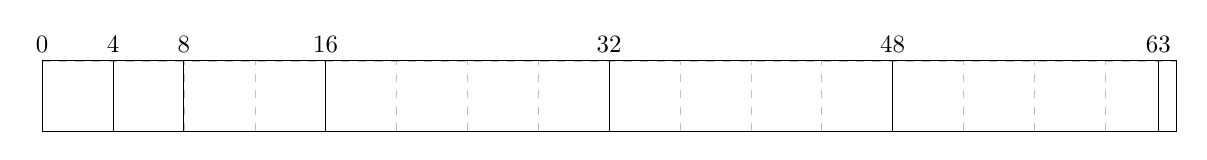
\begin{tikzpicture}[scale=0.9, transform shape]
    
    	\draw[help lines, gray!50, dashed] (0,0) grid(16,1);
    
        % Box for the 64-bit instruction word
        \draw (0,0) rectangle (16,1);

	
         % Bit separators (adjust positions as needed)
        \foreach \x/\label in {0/0, 4/4, 8/8, 16/16, 32/32, 48/48, 63/63} {
            \draw (\x/64*16, 0) -- (\x/64*16, 1); % Scale bit position to 16 cm width
            \node[above] at (\x/64*16, 1) {\label}; % Bit position labels
        }

    \end{tikzpicture}
\end{center}





    %-------------------------------------------------------------------------------------------------------
%-------------------------------------------------------------------------------------------------------
\chapter{Listings test}

\section{CDC Lib}
\newpage

\lstinputlisting[language=c++,style=listingstyle]{\srcinputpath LcsLibraries/LcsCdcLib/LcsCdcLib.h}
\newpage

\lstinputlisting[language=c++,style=listingstyle]{\srcinputpath LcsLibraries/LcsCdcLib/LcsCdcLib.cpp}
\newpage

\section{LCS Runtime Lib}
\newpage

\lstinputlisting[language=c++,style=listingstyle]{\srcinputpath LcsLibraries/LcsRuntimeLib/LcsRuntimeLib.h}
\newpage

\lstinputlisting[language=c++,style=listingstyle]{\srcinputpath LcsLibraries/LcsRuntimeLib/LcsRtLibInt.h}
\newpage

\lstinputlisting[language=c++,style=listingstyle]{\srcinputpath LcsLibraries/LcsRuntimeLib/LcsRtCanBus.cpp}
\newpage

\lstinputlisting[language=c++,style=listingstyle]{\srcinputpath LcsLibraries/LcsRuntimeLib/LcsRtNvmI2C.cpp}
\newpage

\lstinputlisting[language=c++,style=listingstyle]{\srcinputpath LcsLibraries/LcsRuntimeLib/LcsRtSetup.cpp}
\newpage

\lstinputlisting[language=c++,style=listingstyle]{\srcinputpath LcsLibraries/LcsRuntimeLib/LcsRtMsgBus.cpp}
\newpage

\lstinputlisting[language=c++,style=listingstyle]{\srcinputpath LcsLibraries/LcsRuntimeLib/LcsRtAttributes.cpp}
\newpage

\lstinputlisting[language=c++,style=listingstyle]{\srcinputpath LcsLibraries/LcsRuntimeLib/LcsRtEvents.cpp}
\newpage

\lstinputlisting[language=c++,style=listingstyle]{\srcinputpath LcsLibraries/LcsRuntimeLib/LcsRtCommands.cpp}
\newpage

\lstinputlisting[language=c++,style=listingstyle]{\srcinputpath LcsLibraries/LcsRuntimeLib/LcsRtDrvLib.cpp}
\newpage

\lstinputlisting[language=c++,style=listingstyle]{\srcinputpath LcsLibraries/LcsRuntimeLib/LcsRtCore.cpp}
\newpage

\section{Base Station}
\newpage

\lstinputlisting[language=c++,style=listingstyle]{\srcinputpath LcsBaseStation/LcsBaseStation.h}
\newpage

\lstinputlisting[language=c++,style=listingstyle]{\srcinputpath LcsBaseStation/LcsBsCommand.cpp}
\newpage

\lstinputlisting[language=c++,style=listingstyle]{\srcinputpath LcsBaseStation/LcsBsDccTrack.cpp}
\newpage

\lstinputlisting[language=c++,style=listingstyle]{\srcinputpath LcsBaseStation/LcsBsLocoSession.cpp}
\newpage

\lstinputlisting[language=c++,style=listingstyle]{\srcinputpath LcsBaseStation/main.cpp}
\newpage

\section{Block Controller}
\newpage

\lstinputlisting[language=c++,style=listingstyle]{\srcinputpath LcsBlockController/LcsBlockController.h}
\newpage

\lstinputlisting[language=c++,style=listingstyle]{\srcinputpath LcsBlockController/main.cpp}
\newpage

\lstinputlisting[language=c++,style=listingstyle]{\srcinputpath LcsBlockController/LcsBcLogic.cpp}
\newpage

\lstinputlisting[language=c++,style=listingstyle]{\srcinputpath LcsBlockController/LcsBcBlockTrack.cpp}
\newpage

\lstinputlisting[language=c++,style=listingstyle]{\srcinputpath LcsBlockController/LcsBcOccDetect.cpp}
\newpage

\lstinputlisting[language=c++,style=listingstyle]{\srcinputpath LcsBlockController/LcsBcSignalControl.cpp}
\newpage

\lstinputlisting[language=c++,style=listingstyle]{\srcinputpath LcsBlockController/LcsBcTurnoutControl.cpp}
\newpage

\lstinputlisting[language=c++,style=listingstyle]{\srcinputpath LcsBlockController/LcsBcRailCom.cpp}
\newpage


    % Optional: For appendices, bibliography, etc.
    \backmatter             

\end{document}
